
% to choose your degree
% please un-comment just one of the following
\documentclass[bsc,frontabs,twoside,singlespacing,parskip,deptreport]{infthesis}     % for BSc, BEng etc.
% \documentclass[minf,frontabs,twoside,singlespacing,parskip,deptreport]{infthesis}  % for MInf
\usepackage{graphicx}
\usepackage{hyperref}
\usepackage{multirow}
\usepackage{dirtytalk}
\usepackage[utf8]{inputenc}
\usepackage{minted}
\usepackage{hyperref}



\begin{document}

\title{Microbenchmarking Intel Knights Landing}

\author{Alexander Wilson}
 
\course{Computer Science}  

\project{4th Year Project Report}

\date{\today} 

\abstract{
This project investigates how processors with complex memory hierarchies and execution pipelines process instructions and data. This includes evaluating the performance of the memory system of Intel's 2nd Generation Xeon Phi Processor, codenamed Knights Landing. The report covers how instruction latency is measured and how important computer architecture concepts such as pipelining and out-of-order execution are accounted for when conducting measurements. It also covers usage of STREAM, an open-source benchmark for measuring memory bandwidth, on Knights Landing and presents results for latencies and bandwidths of memory components of the Knights Landing Processor. Finally it provides usage instructions for repeating the experiments and running the benchmark suite implemented. \\
\\
The Results and accompanying Discussion also verify performance metrics provided by Intel on the MCDRAM and DRAM Bandwidths, that peak bandwidth of MCDRAM is 400+GB/s.
}

\maketitle

\section*{Acknowledgements}
I would like to thank my supervisor \textbf{Vijay Nagarajan} for his help in supervising this project. Not only did he help me throughout the project, but his teaching in the Computer/Parallel Architecture courses helped me understand fundamental concepts in order to work on this project. \\
\\
I would also like to thank \textbf{all my family} for their extensive support for my education, giving me the time and space I needed to study, and ultimately supporting me pursuing my interests. \\
\\
Finally, I would like to thank my best friend \textbf{Eddy} for always being there to listen to me try to explain my work and being supportive.
\tableofcontents

\pagenumbering{arabic}

\chapter{Introduction}
\section{Project Motivation}
With processors becoming increasingly complex, and the need for large data processing, hardware manufacturers like Intel are producing new and different processors to tackle different problems, using new or different architectural designs. One of the major issues with modern processors is that the memory system is a huge bottleneck in the processor; for example, fetching data from memory takes substantially longer than most arithmetic or logical operations. In order to tackle this issue, complex memory hierarchies of Caches and DRAM are created to try and minimise the latency of a memory access. It is interesting to investigate how processors work, and how these complex memory systems behave, in order to understand how these systems improve program performance.

\section{Project Overview}\label{proj-overview}
The goal of this project is to evaluate the performance of Intel's 2nd Generation Xeon Phi processor's(code-named Knights Landing, or KNL for short) memory system, in order to verify Intel's performance statistics. The project is also about gaining an understanding of how High Performance Computers differ to desktop processors, and an understanding of how parallel processing is achieved in a practical sense. Knights Landing has a complex and interesting memory system, including new memory modules relative to its predecessors. The project scope included measuring the latencies of accessing different regions of memory, namely the L1 Cache, L2 Cache, DRAM, and Intel's new MCDRAM. The project scope also includes investigating how the Cache Coherence system present across the chip behaves, and what the latency of accessing data between Cores is in the different Coherence States. The project scope also includes measuring the bandwidth of the DRAM and MCDRAM, to better understand how data is processed in a High Performance Computing context.

\section{Project Goals Achieved}
From the goals briefly outlined in the \hyperref[proj-overview]{Project Overview} concrete results were obtained for the Bandwidth's of the DRAM and MCDRAM. Concrete results for the latencies of the L1 Cache, L2 Cache, DRAM and MCDRAM. However, the accuracy and validity of the results will be discussed in the \hyperref[chap:discussion]{Discussion Chapter}. Finally, concrete results for the latencies of accessing data in remote Cores was partially obtained for some states, but more work would need to be done to validate the results or obtain other reliable results.

\section{Report Structure}
Following the Introduction; \\
\\
\textbf{Chapter \ref{chap:bground}} will cover background information on computer architecture that will give a general understanding of how processors execute instructions and tackle the long latencies of DRAM accesses using Caches. The Background will also include some rudimentary information on how parallel processors work, and keep their Cache's data coherent across Cores. \\
\\
\textbf{Chapter \ref{chap:knl-arch}} will then outline the architecture of the Knights Landing Processor, including the configurable modes for the L2 Cache, and the MCDRAM. The Chapter will also lightly discuss how the KNL Cores handle Threads, which will be relevant when discussing the measured results. \\
\\
\textbf{Chapter \ref{chap:writing-benchmarks}} is made up of 7 sections:
\begin{enumerate}
    \item Measuring Latency
    \item Measuring Bandwidth
    \item L1 Cache Latency
    \item L2 Cache Latency
    \item DRAM/MCDRAM Latency
    \item Remote Cache Latency(Coherence Miss Latencies)
    \item DRAM/MCDRAM Bandwidth
\end{enumerate}
Section \ref{measuring-latency} discusses the work done in a chronological order, for deciding upon a technique for measuring instruction latency. This section also includes practices used to verify techniques, and the methodology for generating Load instructions. The conclusion of this section is a portable methodology for generating Load instructions, and an approach to measuring instruction execution latency. \\
\\
Section \ref{measuring-bandwidth} briefly introduces the Open Source benchmark program that was used for measuring the bandwidth of the DRAM and MCDRAM. \\
\\
Section \ref{sec:l1-cache-latency} discusses the algorithm of the benchmark program for measuring the latency of an L1 Cache load, which includes a high-level overview of the algorithm, using the conclusions of Section \ref{measuring-latency}(Measuring Latency). \\
\\
Section \ref{sec:l2-cache-latency} discusses the algorithm of the benchmark program for measuring the latency of an L2 Cache load, which includes a high-level overview of the algorithm, using the conclusions of Section \ref{measuring-latency}(Measuring Latency). This section will build upon Section \ref{sec:l1-cache-latency} and note important differences. \\
\\
Section \ref{mcdram-dram-benchmarks-lat} discusses the algorithm of the benchmark program for measuring the latency of a DRAM/MCDRAM load, again this will build upon the previous two sections, noting important differences. \\
\\
Section \ref{coherence-latencies} details how I implemented a multi-threaded benchmark application. It also shows how information highlighted in the Background Chapter (Section \ref{cache-coherence}) is used to place the Processor into a particular state for measuring latencies for accessing data across Cores(into other Caches). \\
\\
Finally, Section \ref{mcdram-dram-benchmarks-bw} discusses what the Bandwidth microbenchmark does, and why it is relevant. This includes discussion of how it was used to ensure the results obtained are valid. \\
\\
\textbf{Chapter \ref{chap:results}} presents the results of running the microbenchmarks from Chapter \ref{chap:writing-benchmarks}. \\
\\
\textbf{Chapter \ref{chap:discussion}} discusses the results obtained, and the validity of the results compared to Intel's published results and results for similar architectures. This Chapter also includes discussion on what could be done to improve the results. \\
\\
\textbf{Chapter \ref{chap:conclusion}} concludes the report, highlighting what work was done, including what was learnt throughout the project. This Chapter will finish by concluding the outcome of the project, including deliverables and further work. \\
\\
\textbf{Chapter \ref{chap:benchmark-suite}} is separate to the main flow of the report, and introduces the Open Source version of the implemented Benchmark Suite, including instructions for usage.

\chapter{Background}\label{chap:bground}
\section{Computer Architecture}
This section will cover design features present in modern processors that are relevant to the scope of this project, specifically in understanding how benchmarks are written.

\subsection{Pipelining}
Pipelining is a technique used in almost all modern processors to commit more instructions per cycle. The technique involves splitting an instruction into stages, and then once any given stage has completed, a new instruction can enter that stage. For example, we could consider a processor to process instructions over 5 stages:
\begin{enumerate}
    \item{{\bf \texttt{IF} - Instruction Fetch} \\ The instruction at the program counter(PC) is fetched from memory, and the PC is incremented.}
    \item{{\bf \texttt{ID} - Instruction Decode} \\ The fetched instruction is decoded, and required values are fetched from general purpose Registers.}
    \item{{\bf \texttt{EXE} - Execution} \\ The arithmetic and logic operations are computed. This includes computation of addresses. }
    \item{{\bf \texttt{MEM} - Memory Access/Branch Completion} \\ Memory is accessed if required.}
    \item{{\bf \texttt{WB} - Write Back} \\ Results of execution are written back to general purpose Registers}
\end{enumerate}
Splitting instruction execution into stages, like the above model, allows the processor to reallocate a given stages resources to a new instruction, once the current instruction has finished using those resources. For example, the processor can begin fetching the next instruction after it has finished fetching the current instruction, but before the current instruction has totally finished being executed. This means that in the ideal situation, our model can have 5 instructions in flight, and given that each stage costs one cycle, potentially committing an instruction every cycle. It is important to note that in practice, this is likely won't happen, for example, complex arithmetic such as divisions will take multiple cycles to complete the \texttt{EXE} stage.

%%%%%%%%%%%%%%%%%%%%%%%%%%%%%%%%%%%%%%%%%%%%%%%%%%%%%%%%%%%%%%%%%%%%%%%%%%%%%%%%%

\subsection{Out-Of-Order Execution}
Out of order execution is a technique used in processors to increase the efficiency of the pipeline. The processor can re-order instructions to make more efficient usage of the different stages. For example, if you have a complex division instruction, followed by a few simple addition instructions, the processor could push the additions into the pipeline first, and the division last, so that the pipeline doesn't halt or bottleneck at the \texttt{EXE} stage while waiting for the complex division to be calculated, leaving other instructions halted in flight behind it. Out-Of-Order execution is complex, and if the CPU were to re-order dependent instructions, it would have other systems in place to handle instruction dependencies. An example of such a dependency would be:
\begin{center}
\verb
x = a / b
\\
\verb
y = x + 5
\end{center}
Where the value of \texttt{y} cannot be calculated until the result of \texttt{x} has been calculated, and so \texttt{y = x + 5} may hang at the \texttt{ID} stage, essentially halting the pipeline. However pipelining techniques to tackle instruction dependencies are out of the scope of the project, but it is important to understand that modern processors may re-order instructions.

%%%%%%%%%%%%%%%%%%%%%%%%%%%%%%%%%%%%%%%%%%%%%%%%%%%%%%%%%%%%%%%%%%%%%%%%%%%%%%%%%

\subsection{Caching}
\subsubsection{Motivation}
Moore's Law states that the number of transistors that could be fit onto a computer chip would scale up by a factor of five, every five years. To begin with, the extra transistors on the chips were used for created logical units that could compute logical/arithmetic operations quicker, however it was soon realised that despite processors being able to process arithmetic with a latency as low as a single cycle, actually retrieving the data to perform the logical/arithmetic operations on was becoming a huge bottleneck. For example; the \texttt{EXE} stage of the pipeline could process simple addition operations in a single cycle, but retrieving the additions operands can cost up to a few hundred cycles to retrieve from memory, and so memory latency became a significant bottleneck in the pipeline.
\subsubsection{Solution}
The solution to this problem has not just been to throw more hardware at main memory, but to use the new transistors on chips to create a memory hierarchy that caches and pre-fetches data that is likely to be used. Most general purpose CPU's today have a two to three level cache hierarchy, with level one being the smallest and closest to the processor cores, and level 3 being the biggest. When referring to different levels of caches in a processor, \texttt{L1} is used to refer to the level one cache; likewise \texttt{L2} to refer to the level two cache.
\par
\subsubsection{Cache Behaviour}
Each processor model will have its own unique cache architecture. However it is typical for an \texttt{L1} cache to exist spatially close to a single core, and be unique to that core. Some architectures have \texttt{L2} caches unique to a core, however, it is more common that the \texttt{L2} cache is shared among cores. There are two ways that caches are designed to be indexed; Direct-Mapping and Set-Associative.
\begin{itemize}
    \item{
        {\bf Direct Mapping} \\
        Each line in memory is mapped to a specific line in the cache. If memory has \texttt{M} lines, and our cache has \texttt{C} lines, where \texttt{C < M}, memory line \texttt{m} is located in the cache at line \texttt{m modulo C}\\
        This has the advantage of being quick to access, as you simply look up the line in the cache where the address you wish to read/write to would exist, and if the tag of the cache-line and your address match, you have found your data quickly. \\
        This method can incur cache thrashing. Cache thrashing is when useful data is evicted from the cache. For example, say you have two variables in memory, and they both map to the same cache line, the cache could be evicting and replacing this line potentially many times depending on the nature of the program and its use of program variables/memory. \\
        \\
        Figure \ref{fig:dir-map}, shows how lines in memory are mapped in a cyclic fashion to lines in the cache.
    }
    \begin{figure}[h]
        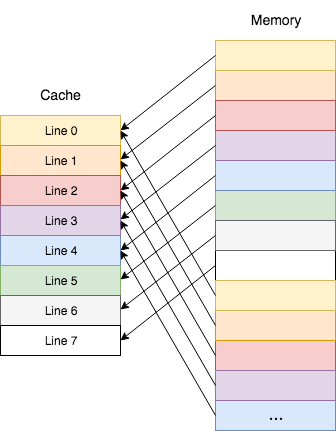
\includegraphics[width=4cm]{Results/direct_mapped.png}
        \centering
        \caption{Direct Mapped Cache Diagram}
        \label{fig:dir-map}
    \end{figure}
    
    \item{
        {\bf Set Associative} \\
        An N-way set associative cache is a cache that is split into sets containing N lines. Therefore if we have a cache with 32 lines, and it is 4-way set associative, then our cache has 8 sets, each containing 4 lines. Memory is mapped to set-associative caches similarly to direct mapping, but instead of mapping a line in memory to a specific line in a cache, it is mapped to a set in a cache, and then the contents of the sets are managed using a cache replacement policy(such as least-recently-used (LRU), first-in-first-out or random-replacement). This also allows for a fully-associative cache, where there is only 1 set, where all cache lines are stored/evicted based on a replacement policy. \\
        This has the advantage of dealing with cache trashing, where multiple lines can exist in the cache at the same time, that would not exist simultaneously in a Direct Mapped cache. \\
        In the case of a fully-associative cache, there is a large overhead in searching the cache for the data that you want, and so in practice, N-way set associative caches are often used in general purpose CPU's to get the best of both Direct Mapped and Fully Associative mappings. But that is not to say that there are no use-cases for Direct Mapped caches. \\
        \\
        Figure \ref{fig:set-assoc}, shows how lines in memory are mapped to one \textbf{set} in the cache. It's important to note that the items within a \textbf{set} are evicted based on the architectures chosen replacement policy. 
    }
    \begin{figure}[h]
        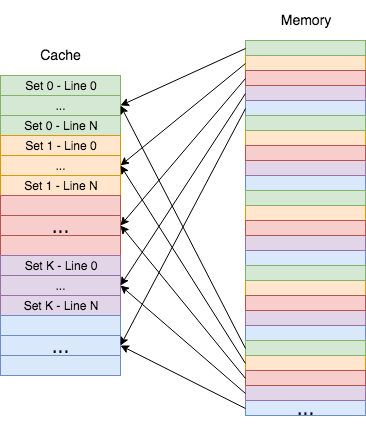
\includegraphics[width=6cm]{set_assoc.png}
        \centering
        \caption{N-way Set Associative Cache Diagram}
        \label{fig:set-assoc}
    \end{figure}
\end{itemize}

It is also important to note that a cache line can vary in size depending on architecture, but it is common for cache lines to be 64B, as it is affordable to transport 64B between caches and memory while exploiting program spatial locality\footnote{Program Spatial Locality: Programs often access nearby memory addresses. For example, incremented indexes in an array.}.

\newpage

\section{Parallel Architectures}

\subsection{Cache Coherence}\label{cache-coherence}
Modern Processors are often Multi-Core systems, with each Core having its own Cache System. Figure \ref{fig:parallel-cpu} illustrates a simple Chip which may consist of 4 Cores connected to a Bus and DRAM. \\
\begin{figure}[!h]
    \centering
    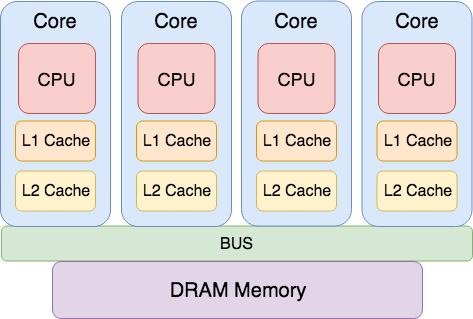
\includegraphics[width=8cm]{Parallel.png}
    \caption{Parallel Chip System}
    \label{fig:parallel-cpu}
\end{figure} \\
It is easy to envision that programs would exist where data can be processed in a parallel fashion; i.e. where the majority of the processing does not need to be done in any particular order. Such a scenario would mean that all those processing tasks can be run simultaneously on different cores. Cache Coherence Protocols are a means of tracking where data exists in the different Cores, and ensuring that only one \textbf{value} of a particular piece of data exists. In practice, Coherence Protocols offer write serialisation\footnote{Write-Serialisation: The notion of all cores in a system mutually agreeing on the order of variable writes.} and write-propagation\footnote{Write-Propogation: The notion that the outcome of the write must eventually reach other cores.} in many-core systems, as they essentially abstract away the existence of multiple Caches, and create a system where there appears to be only one large Cache. Coherence Protocols are implemented using States, which track where the data exists, if it has been modified, and if it's valid.

\subsection{MESI Protocol}\label{sec:mesi-protocol}
The \texttt{MESI} Protocol is a Cache Coherence protocol that is based on the following four states:
\begin{itemize}
    \item \textbf{Modified} \\
    A line that exists in Modified State in a Cache guarantees that it is the only valid version of this Line across all Cores, where the Line is dirty\footnote{Dirty Line: A line which has been modified and its value not written back to memory yet.}.
    \item \textbf{Exclusive} \\
    A line that exists in Exclusive State in a Cache guarantees that it is the only valid version of this Line across all Cores, where the Line is NOT dirty.
    \item \textbf{Shared} \\
    A line that exists in Shared State in a Cache guarantees that there \emph{may} exist other unmodified copies of this Line in one or more of the other Cores.
    \item \textbf{Invalid} \\
    A line can exist in the Invalid State in a Cache, meaning that its value has been invalidated. A line can be invalidated by another Core modifying a line, which invalidates other copies of the same Line.
\end{itemize}
In the most simple case, these protocols are enforced over the means of "snooping" the bus medium. This means that there are controllers on each Core that are constantly listening on the Bus, can send messages on the Bus, and react to messages sent on the Bus. Figure \ref{fig:mesi-state} shows the State Diagram of the \texttt{MESI} Protocol. Although the State Diagram is quite complex, it is important to note that upon a \textbf{Remote Core} performing a Write, all other Cores Invalidate their Line, and that regardless of State, if a \textbf{Local Core} performs a Write, it always enters the Modified State. This shows that only one value per data can exist in a Coherent Cache System. 

\begin{figure}[!h]
    \centering
    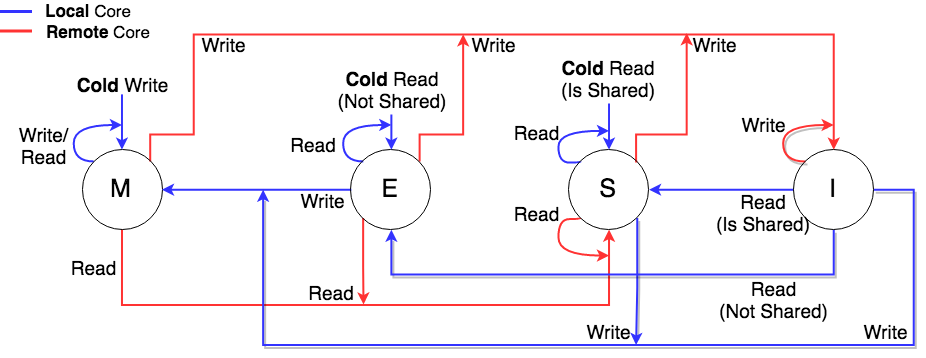
\includegraphics[width=15cm]{MESI.png}
    \caption{\texttt{MESI} Protocol - State Diagram}
    \label{fig:mesi-state}
\end{figure}

An example of how the State Diagram in Figure \ref{fig:mesi-state} can be interpreted: \\
\\
Say we have 4 Processors: [P0, P1, P2, P3], and we use the following format to denote P1 performing a Read to Line 5: \texttt{P1 R 5}, and P3 performing a Write to Line 1000: \texttt{P3 W 1000}.
If we want to generate a scenario where Processors 0 and 1 both own line 50 in the Shared State, we can do the following:
\begin{center}
\verb
P0 R 50
\\
\verb
P3 R 50
\end{center}
Using Figure \ref{fig:mesi-state}, we look at P0, it performs a "Cold Read" to Line 50, and so now P0 owns Line 50 in Exclusive State. When P3 performs a "Cold Read" to Line 50, the State transitioning from "\textbf{Cold} Read (Is Shared)" triggers, and P3 now owns Line 50 in the Shared State. Because this Read is communicated via the bus, it would, in fact, be P0 that supplies P3 with the Line, and P0 would observe a "Remote Read", which following the State Diagram, changes P0's Exclusive Line 50, to a Shared Line 50. Now both P0 and P3 own Line 50 in the Shared state. Later sections that discuss Coherence Latencies will make reference to the \texttt{MESI} and \texttt{MESIF} Protocols in order to get data into certain states in a benchmark setting.

\subsection{MESIF Protocol}\label{sec:mesif-protocol}
The \texttt{MESIF} Protocol is an extension and modification of the \texttt{MESI} protocol, that adds the new Forward State, and alters the purpose of the Shared State. In \texttt{MESIF}, a line that exists in Shared State cannot be copied, and instead, it holds that a single instance of the Shared Line will be held in the Forward State\cite{mesif-paper}, and that the Core that holds the Line in Forward State shall be responsible for forwarding the Data. There is also no guarantee that the Line in Forward State will be spatially close to the requesting Core. The motivation for this additional Forward state, is to reduce traffic on the Bus, because in MESI, if a Core requests data that exists in multiple other Cores in Shared State, all the Cores will respond to the request. However, in the MESIF protocol, the Core that contains the Shared Line in Forward State is the only Core responsible for responding to the Request. This is enough of an understanding of the \texttt{MESIF} Protocol that is required for the scope of this project, as we will only be interested in setting up Cores to own lines in different Coherence States.

\chapter{Understanding KNL Architecture}\label{chap:knl-arch}
This chapter will outline the KNL Architecture, detailing what needs to be known to understand how the benchmarks work.
\section{Chip Layout}
\begin{figure}[h]
    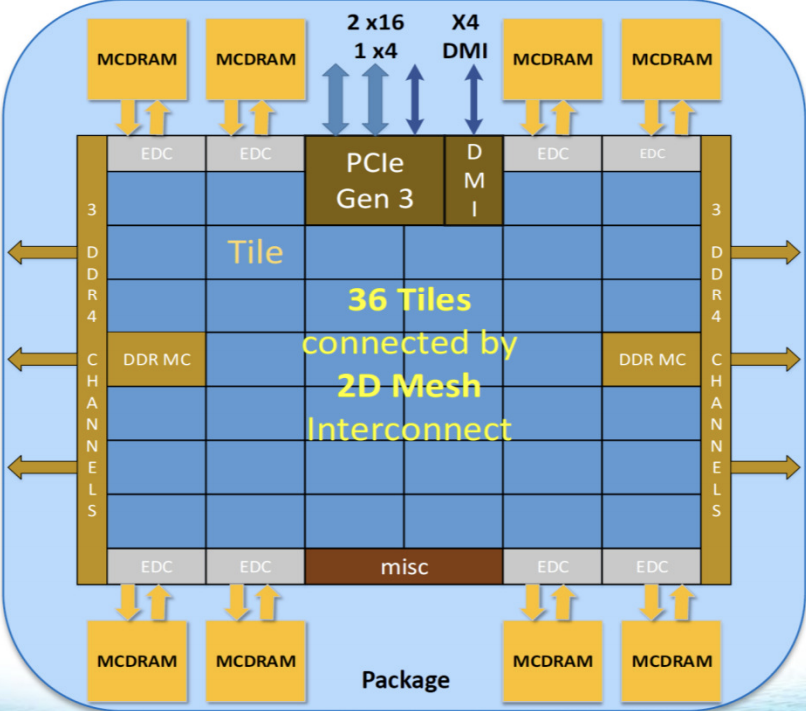
\includegraphics[width=10cm]{KNL_Overview.png}
    \centering
    \caption{KNL Chip Layout}
    \protect\cite{intel_pres}
    \label{fig:chip-overview}
\end{figure}
Figure \ref{fig:chip-overview}, shows a top-down view of the architecture of the KNL chip. The chip is a mesh of 36 tiles.

\subsection{Tile}
A tile consists of:
\begin{itemize}
    \item 2 x CPU Cores:
    \begin{itemize}
        \item \texttt{32KB L1} Instruction Cache \ \ \ \ \ \ \texttt{8-way} set-associative, \texttt{64B} cache lines
        \item \texttt{32KB L1} Data Cache \ \ \ \ \ \ \ \ \ \ \ \ \ \ \ \ \texttt{8-way} set-associative, \texttt{64B} cache lines
    \end{itemize}
    
    \item 1 x L2 Cache
    \begin{itemize}
        \item \texttt{1MB} Cache shared between Cores.
        \item \texttt{16-way} set-associative, \texttt{64B} cache lines
        \item Performs a single \texttt{read} in \texttt{1 cycle}.
        \item Performs a single \texttt{write} in \texttt{2 cycles}.
        \item L2 Cache \textbf{coherent} with all other tiles L2 Caches.
    \end{itemize}
    
    \item 1 x Caching/Home Agent
    \begin{itemize}
        \item Distributed Tag Directory to keep \texttt{L2 Caches} coherent across tiles.
    \end{itemize}
\end{itemize}
\subsection{L2 Cache}
The mesh of tiles creates a distributed \texttt{L2} Cache. This mesh is configurable in three different modes:
\begin{itemize}

    \item \textbf{All-to-All} \\
    All of the \texttt{L2} Address space is uniformly distributed across all tiles. This means that any given core can access data in the \texttt{L2} Cache of any other tile. A typical miss in All-to-All mode starts with a Core missing in its \texttt{L1} Cache, it then checks its own tiles \texttt{L2} Cache, and upon missing, checks the \textbf{distributed} directory. After missing in the \textbf{distributed} directory, the request is forwarded to MCDRAM/DRAM(Depending on configuration).\\
    Most general mode, so relatively lower performance.
    
    \item \textbf{Quadrant} \\
    The Chip is divided into four virtual quadrants. Addresses are hashed to a directory in the same quadrant. This means that a core can access data in the \texttt{L2} Cache of any other tile in the same virtual quadrant. A typical miss in Quadrant mode starts with a Core missing in its \texttt{L1} Cache, it then checks its own tiles \texttt{L2} Cache, and upon missing, checks the \textbf{quadrant} directory. After missing in the \textbf{quadrant} directory, the request is forwarded to MCDRAM/DRAM(Depending on configuration).\\
    This mode has a lower latency, and higher bandwidth relative to \texttt{All-to-All}. Quadrants are transparent to software.
    
    \item \textbf{Sub-NUMA Clustering}\label{snc4-explained} \\
    The Chip is divided into four quadrants. Each exposed to the OS as a separate NUMA\footnote{NUMA: Non-Uniform Memory Access; The idea that different cores have their own physical memory.} domain. To the operating system, this looks analogous to a 4 socket Xeon(server) processor. A typical miss in Sub-NUMA mode starts with a Core missing in its \texttt{L1} Cache, it then checks the \textbf{quadrant} directory. After missing in the \textbf{quadrant} directory, the request is forwarded to MCDRAM/DRAM(Depending on configuration). \\
    This mode has the lowest latency of all three modes, due to the nature of NUMA and spatial locality, but requires software support to handle the distributed memory.
    
\end{itemize}

\subsection{MCDRAM}
The KNL Chip includes a new layer of high-bandwidth memory that is spatially close to the chip, but has a higher access latency compared to DRAM. Intel coined MCDRAM is 16GB of DRAM built into the chip, with three configurable modes:

\begin{itemize}
    \item \textbf{Cache Mode} \\
    The 16GB of memory is used to cache DRAM. This is completely transparent to software, and so any memory address that doesn't exist in the \texttt{L1} or \texttt{L2} Cache's is directed to MCDRAM next. When considering access latencies, visiting MCDRAM is already more costly than visiting DRAM, but missing in MCDRAM also then requires a further look up to main memory. This effectively means that Cache Mode is best used for frequently used contiguous\footnote{Contiguous Memory: Memory that exists spatially next to each other.} memory, as data can be pulled into \texttt{L2} and \texttt{L1} Caches with fewer accesses to memory.
    
    \item \textbf{Flat Mode} \\
    The 16GB of memory is used to extend DRAM, essentially extending its address space. This mode requires programs to be aware of this configuration, and address memory appropriately
    
    \item \textbf{Hybrid Mode} \\
    The 16GB of memory can be used to both extend DRAM, and cache it. It can be configured to use either 25\% or 50\% of the 16GB as a DRAM Cache, with the rest extending DRAM. This has the benefit of extending DRAM, and also caching data that is frequently used.
\end{itemize}

\section{Threading}\label{knl-threading}
Intel's Presentation\cite{intel_pres} on the Knights Landing chip highlights the Core's multithreading capabilities. It is important to note that Core's resources are shared or dynamically re-partitioned among threads, so stalls will be incurred when thread contexts are switched. These observations will be particularly noticeable when discussing our results.

\chapter{Writing the Microbenchmarks}\label{chap:writing-benchmarks}
This chapter will talk about the different approaches to benchmarking latencies and bandwidths of different memory components, and tackling obstacles that would prevent accurate or reliable results. It will then describe the how the discoveries made were used to create microbenchmarks for the L1 Cache, L2 Cache, DRAM, and MCDRAM.

\section{Measuring Latency}\label{measuring-latency}
For measuring latencies, a reliable timing technique must be used that is accurate enough to time fine-grain operations to nanosecond precision. At a high-level, the latency measuring technique involves taking a reading of time before and after an instruction(s) of interest, and calculating the difference between said times, minus the overhead of timing. It is also important to make sure that we are timing the desired instructions.

\subsection{Hardware Support/Tools}
In order to perform high-precision latency benchmarks, we must have hardware support and tools that allow us to take fine-grain measurements of time, as standard c++ timing libraries cannot provide the precision required to gain any meaningful results.

\subsubsection{Timestamp Counter (TSC)}
The Timestamp Counter (TSC) is a measuring "device" that allows us to get information on the current cycle-count of the processor. Traditionally, the TSC was a register that existed in each Core. The value in the register would be incremented every cycle, and therefore could be read and the value returned could be used to count the number of cycles elapsed. This was useful for programmers to benchmark how their code would perform in terms of cycles spent, but would not provide a portable solution for measuring wall-time\footnote{Wall-Time: Real-world time.} since wall-time is a combination of cycles spent and core frequency. \\
\\
Calculating the wall-time using the traditional TSC becomes increasingly difficult when we consider that Intel uses technologies to change Core's frequencies dynamically (for purposes such as power-saving). Since the TSC is also local to each individual Core, it cannot be used to measure code that runs concurrently across multiple cores. Modern Intel CPUs provide access to an "invariant TSC", which increments at set intervals, meaning it can be used for measuring wall-time. Knights Landing does have an invariant TSC, and as such can be used in our microbenchmarks. \\
\\
Refer to Appendix A.1 for information on what your Processor's TSC support is.

\subsubsection{Assembly Instructions/Flags}
In order to make use of our hardware tools, we must have appropriate Assembly Instructions. The three Instructions of interest to this project are:
\begin{itemize}
    \item{
        {\bf \texttt{CPUID}\cite{cpuid_spec}} \\
        This instruction is a serialising instruction, which guarantees: \\
        "any modifications to flags, registers, and memory for previous instructions are completed before the next instruction is fetched and executed."
    }
    \item{
        {\bf \texttt{MFENCE}\cite{mfence_spec}} \\
        Assembly Instruction/Flag which guarantees that all loads/stores prior to it have been globally retired. Meaning that the resulting memory operation is visible globally.
    }
    \item{{\bf \texttt{RDTSCP}\cite{rdtscp_spec}} \\
    Hardware supports a call to reading the TSC that waits until all previous instructions have finished executing and are globally retired via the \texttt{RDTSCP} Instruction. But is NOT a serialising Instruction.}
\end{itemize}
As the techniques for timing are explored we will see the relevance of all the above Assembly Instructions.

\subsection{Important Considerations}\label{timing-considerations}
Despite having good hardware tools, there are still some issues that must be considered and tackled in order for our chosen timing technique to be valid. \\
\\
The three core considerations are:
\begin{enumerate}
    \item Core Affinity: Process/Thread Placement
    \item Compiler Optimisations
    \item Out-of-Order Execution
\end{enumerate}

\subsubsection{Core Affinity}
Core affinity is the notion of binding a Process or Thread to a Core or range of Cores on a system. This is an important consideration as the  TSC is Core Specific. Therefore we want to make sure that we pin our threads to a single core, to ensure that our TSC reads are reading the same register, as there is no guarantee that all TSC Registers across cores will have the same value. It also prevents us accidentally measuring the latency of migrating a process/thread to another Core.\\
\\
The Linux c++ library \texttt{sched.h} provides a library for scheduling, and StackOverflow user Ankur Chauhan provided a clean implementation\cite{corepin_src} for pinning the current thread to a specific Core using \texttt{sched.h}. The implementation was tested to ensure it works appropriately and subsequently it was used within the microbenchmarks.

\subsubsection{Compiler Optimisations}\label{compiler-optimisations}

All compilation is done using the following command to ensure that the features of c++ we require are available:
\begin{center}
    \texttt{prog.cpp -std=c++0x [-pthread] -o coherence\_latencies.o}
\end{center}
It is important to consider optimisations that the Compiler may use when generating the executable. To ensure that critical sections of the microbenchmarks are not optimised out, we can make use of the \texttt{volatile} keyword, which tells the compiler not to remove the code, in the event that it detects it to be dead code. Later sections will show how the \textbf{volatile} keyword is used to ensure code is not removed.

\subsubsection{Out-of-Order Execution}\label{ooo-exec}
Out-of-Order Execution (OoOE) was introduced in Section \ref{ooo-exec}, and is a major obstacle in writing correct microbenchmarks. If the microbenchmark code is not crafted carefully, instructions will be shuffled around by the processor to allow the code to stream through the pipeline quicker, and the instructions that the microbenchmark intends to time, may not be the timed instructions. We will see in Section \ref{timing-technique} how the development of the timing component of our microbenchmarks takes OoOE into account.

As I discuss the methodology for arriving at the chosen timing technique, I will refer to these considerations and how they affected the chosen technique.

\subsection{Timing Technique}\label{timing-technique}
This section will progressively describe the chosen timing technique with reference to the considerations in Section \ref{timing-considerations}, and how the timing technique was verified.

\subsubsection{Timing Verification}
In order to have a timing mechanism that could be reliably used in a microbenchmark, it was important not just to experiment with different timing techniques, but to be able to verify our experiments using known values. \\
\\
Using Agner Fog's "Instruction Tables"\cite{inst_tables}, which details cycle latency for standard x86 Instructions on different CPU Architectures, a test suite coined the "Sanity Tests" was crafted to ensure that when using a given timing mechanism, it would return valid latencies. These Sanity Tests would also perform an "overhead" test to ensure that the overhead of the timing mechanism was consistent and reliable, otherwise, it would not be possible to subtract the overhead from our measured latency. \\
\\
The Sanity Tests timed 1000 runs of the following instructions, and the returned latencies could be compared to Fog's table entry for the Knights Landing processor:
\begin{itemize}
    \item{{\bf \texttt{DIV}} \\
        The Division Instruction was expected to have a latency of \textbf{29-95 Cycles}.
    }
    \item{{\bf \texttt{PAUSE}} \\
        The PAUSE Instruction was expected to have a latency of \textbf{25 Cycles}
    }
    \item{{\bf \texttt{F2XM1}} \\
        The F2XM1 Instruction was expected to have a latency of \textbf{100-400 Cycles}.
    }
\end{itemize}

\underline{\textbf{Sanity Test Algorithm:}}\label{sanity-test-algo} \\
\begin{minted}[linenos]{py}
latencies = [0] * 500
for i in range(0,1000):
    start = start_timestamp()
    # Timed Instruction, empty if timing Overhead.
    end   = end_timestamp()
    latencies[(end - start)]++

for idx, latency in enumerate(latencies):
    print str(idx) + " Cycles Occurred " + str(latency) + " Times"
\end{minted}


\subsubsection{BenchIT Solution\cite{benchit_src}}\label{benchit-disc}
The initial timing mechanism tested was based on the source code of the BenchIT microbenchmark suite:
\begin{minted}{cpp}
unsigned long long timestamp()
{
  if (!has_rdtsc()) return 0;
  __asm__ __volatile__("rdtsc;": "=a" (reg_a), "=d" (reg_d));
  return (reg_d<<32)|(reg_a&0xffffffffULL);
}
\end{minted}
This code produces a simple piece of assembly that reads from the TSC and stores the upper 32-bits into one register, and the lower 32-bits into another register, then returns a 64bit integer result. The BenchIT solution also includes a code snippet which essentially "warms-up" the \texttt{RDTSC} instruction, which when included in the microbenchmarks, improved consistency of the results across runs.\\
\\
This is a good foundation on which to build a timing mechanism but it does not inherently tackle the issue of \texttt{OoOE}, so it must be modified to include some serialising instruction(s).

\subsubsection{Serialising via \texttt{CPUID}}
Building upon the solution provided by BenchIT, experiments with placing \texttt{CPUID} Instructions around the \texttt{RDTSC} call were experimented with (including solutions provided in an Intel HPC Guide\cite{intel_hpc_guide}) and run through the Sanity Tests, however, none of the experiments produced reliable, consistent or correct results.

\subsubsection{Intel's Benchmark Code Execution Time\cite{code_exec_times}}
In further research, a paper\cite{code_exec_times} by Gabriele Paoloni deep dives an approach to benchmarking code execution time. The proposed timing technique for systems that support the \texttt{RDTSCP} instructions is as follows:
\begin{minted}[linenos]{cpp}
asm volatile (
    "CPUID\n\t"
    "RDTSC\n\t"
    "mov %%edx, %0\n\t"
    "mov %%eax, %1\n\t"
    :"=r" (cycles_high), "=r" (cycles_low)
    ::"%rax", "%rbx", "%rcx", "%rdx"
);
/* Code to time here - Critical Section */
asm volatile(
    "RDTSCP\n\t"
    "mov %%edx, %0\n\t"
    "mov %%eax, %1\n\t"
    "CPUID\n\t"
    :"=r" (cycles_high1),"=r" (cycles_low1)
    ::"%rax", "%rbx", "%rcx", "%rdx"
);
\end{minted}
An explanation of the code is as follows (also available on Pages 16-17 of \cite{code_exec_times}):
\begin{enumerate}
    \item \textit{Line 2} calls \texttt{CPUID} which ensures that any code prior to our Critical Section finishes execution, and cannot be executed within our Critical Section or Timing Mechanism.
    \item \textit{Line 3} calls \texttt{RDTSC}, which reads the TSC into the \textbf{eax} and \textbf{edx} registers.
    \item \textit{Line 4}, \textit{Line 5}, and \textit{Line 6} then store the \textbf{eax} and \textbf{edx} values to memory.
    \item \textit{Line 7} Informs the Compiler which registers are in use (clobbered) for its own internal knowledge.
    \item \textit{Line 9} will then contain the Critical Section of code which is to be benchmarked. It is advisable to have the code in-lined here in order to ensure that the overhead of a function call is not measured.
    \item \textit{Line 11} calls \texttt{RDTSCP} which ensures that all the previous instructions have finished executing, and then reads the TSC into the \textbf{eax} and \textbf{edx} registers.
    \item \textit{Line 12}, \textit{Line 13}, and \textit{Line 15} then store the \textbf{eax} and \textbf{edx} values to memory.
    \item \textit{Line 14} calls \texttt{CPUID} which ensures that any code prior has finished executing and that no proceeding code will be executed prior to \textit{Line 14} which would poison our timing mechanism.
    \item \textit{Line 16} Informs the Compiler which registers are in use (clobbered) for its own internal knowledge.
\end{enumerate}
This technique was run against the \textit{Sanity Check} and produced the most consistent results of all techniques. And the measured latencies aligned with ballpark figures.\\
\\
Table \ref{fig:sanity-results} shows the results of timing each of the following instructions: \{\texttt{DIV, PAUSE, F2XM1}\} 1,000 times, and counting the observed latencies in each run:
% Sanity Check Results #1
\begin{table}[!h]
\begin{center}
\caption{\textit{Sanity Check} Results - 1,000 Runs Per Instruction}
\label{fig:sanity-results}
\begin{tabular}{ |c||c|c|c|c| } 
    \hline
    Latency Observed & Overhead & DIV(29-95) & PAUSE(25) & F2XM1(100-400) \\
    \hline
    39 Cycles  & 822 & 0   & 0   & 0   \\
    52 Cycles  & 178 & 0   & 0   & 0   \\
    65 Cycles  & 0   & 0   & 847 & 0   \\
    78 Cycles  & 0   & 691 & 153 & 0   \\
    91 Cycles  & 0   & 309 & 0   & 0   \\
    377 Cycles & 0   & 0   & 0   & 537 \\
    390 Cycles & 0   & 0   & 0   & 462 \\
    \hline
\end{tabular}
\end{center}
\end{table}

\newpage

As mentioned, Table \ref{fig:sanity-results} shows that we are getting consistent ballpark figures for our latency measurements, but not precise values. If we look purely at the set of Latencies observed, we can see that the latencies we observe are all multiples of 13. This indicates that our timing technique can only take a measurement every 13 Cycles. It can also be observed that there is always a portion of our observations (let us call it an anomaly) that is off by 1 measurement unit (13 Cycles being our "measurement unit"). Regardless of how many trials we run for each instruction, be it 1,000,000 or 50; this anomaly always exists.


\subsubsection{Further Analysis of Intel's Solution}

With a benchmarking technique that provides consistent figures, further analysis had to be done to understand how we could improve the accuracy of the results. \\
\\
As observed, the results were consistent but inaccurate. This was due to all observed latencies being multiples of 13 Cycles. It was hypothesised that this issue exists as a result of an alignment issue with our timing technique and the instruction being timed, and experiments were conducted with timing different numbers of the same Instruction consecutively. For example, instead of timing one single \texttt{PAUSE} Instruction, we could instead time \texttt{N} consecutive \texttt{PAUSE} Instructions and divide our latency (without the overhead) by \texttt{N}. \\
\\
After trialling various values for the number of consecutive Instructions, it was found that 13 Instructions yielded results where the observed Latency was most similar to the actual Latency. Figure \ref{fig:measure-alignment} shows a rough pictorial representation of the hypothesis/observation in action, where green blocks represent a 13 Cycle interval, and the blue blocks represent a 25 Cycle \texttt{PAUSE} instruction:
\\
\begin{figure}[h]
    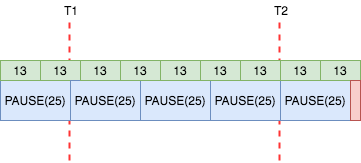
\includegraphics[width=12cm]{MeasureAlignment.png}
    \centering
    \caption{\texttt{PAUSE} Measuring Alignment}
    \label{fig:measure-alignment}
\end{figure}
\\
Although Figure \ref{fig:measure-alignment} does not perfectly ratio the size of our 13 Cycle blocks to our 25 Cycle PAUSE Instructions, thinking about the concept shows that at time \texttt{T1}, our \texttt{PAUSE} Instruction that we are measuring has completed, but due to the accuracy of our timing mechanism, we mark the end of its completion as 26 Cycles (after the second 13 Cycle block). However, we see that after so many Instructions, that at time T2, the end of a 13 Cycle block aligns with the end of a \texttt{PAUSE} Instruction. It makes sense that after performing 13 consecutive \texttt{PAUSE} Instructions, that the end of the final \texttt{PAUSE} would align with the of a 13 Cycle block. And that in general, for an Instruction \texttt{X} with a consistent Latency of \texttt{Y} Cycles, queuing 13 of \texttt{X} consecutively will result in \texttt{Y} 13 Cycle blocks aligning with the final \texttt{X} Instruction.  \\
\\
We can use this fact to take measurements to an accuracy of 1 Cycle, simply by chaining multiple of the measured Instructions together in multiples of 13 within the timing measurements. Our revised \textit{Sanity Test} now includes instructions with a lower expected latency, to test this hypothesis, and the results are as follows, with the overhead remaining the same at 39 Cycles:

\begin{table}[!h]
\begin{center}
\caption{\textit{Sanity Check} Revised Results - 1,000 Runs Per Instruction}
\label{fig:sanity-results-2}
\begin{tabular}{ |c||c|c|c| } 
    \hline
    Latency Observed & CWDE(1) & PAUSE(25) & CWD(7) \\
    \hline
    1 Cycles   & 1000 & 0   & 0   \\
    6 Cycles   & 0    & 0   & 312 \\
    7 Cycles   & 0    & 0   & 685 \\
    25 Cycles  & 0    & 813 & 0 \\
    26 Cycles  & 0    & 185 & 0   \\
    \hline
\end{tabular}
\end{center}
\end{table}

Table \ref{fig:sanity-results-2} shows that we get much more accurate results for each Instruction, however, in some Instruction's cases, we still have this anomaly that exists. This could be due to various reasons, each of which are difficult to verify. Some examples of reasons that were considered but not investigated are:

\begin{enumerate}
    \item{{\bf Assembly to Micro-Op Translation} \\
        Despite writing Assembly Instructions, x86 Instructions are in fact broken down further into Micro-Operations, this is advantageous to the processor as it allows the CPU to re-order 'stages' of an Instruction. This is difficult to investigate as it is Instruction specific, and for the scope of this project, we are interested mostly in Load Instructions, for which there is not much documentation for.
    }
    \item{{\bf Pipeline Optimisations/Considerations} \\
        What Intel's processors do internally is proprietary information, and it is not possible to know exactly what is going on inside the Processor or pipeline, it may be that for some Instructions (for example \texttt{CWD}) in Table \ref{fig:sanity-results-2}) that the Processor is able to perform an optimisation that can cut the Cycle time for multiple or consecutive identical Instructions.
    }
\end{enumerate}

%%%%%%%%%%%%%%%%%%%%%%%%%%%%%%%%%%%%%%%%%%%%%%%%%%%%%%%%%%%%%%%%%%%%%%%%%%%%%%%%%

\subsection{Generating Loads}\label{sec:gen-loads}
It is important to consider how we will generate Load Instructions. It would be possible to use a simple piece of \texttt{c++} code such as:
\begin{minted}{cpp}
volatile int temp;
temp = data[idx];
\end{minted}
To generate a Load to \texttt{data[idx]}, however, this would also generate a Store to \texttt{temp} which would be behaviour we do not wish to time when conducting Load Latency Benchmarks. Therefore we must use the following code snippet to generate a load instruction:
\begin{figure}[!h]
    \centering
    \begin{minipage}{0.4\textwidth}
    \begin{minted}{cpp}
asm volatile (
    "\n\tmov %%eax, %0"
    "\n\tMFENCE"
    ::"r"(data[0]):
);
    \end{minted}
    \end{minipage}
    \caption{Load Instruction \texttt{c++} Inline Assembly }
    \label{fig:load-inst-code}
\end{figure}

If we look at the Assembly generated by the compilation of Figure \ref{fig:load-inst-code}:
\begin{figure}[!h]
    \centering
    \begin{minipage}{0.4\textwidth}
    \begin{minted}[linenos]{asm}
mov eax, DWORD PTR [rbp-262272]
mov %eax, eax
MFENCE
    \end{minted}
    \end{minipage}
\end{figure} \\
\texttt{Line 1} shows the Load Instruction that we will wish to time, which moves a Line from Memory into a Register, the \textbf{eax} (without the proceeding '\%') indicates that an arbitrary register will be allocated. \texttt{Line 2} shows a \texttt{MOV} Instruction generated by the compiler that would move the result of \texttt{Line 1} into the \texttt{eax} Register. We do not wish to time this second \texttt{MOV} Instruction, but can account for it when calculating our overhead. And \texttt{Line 3} shows the \texttt{MFENCE} flag that will ensure the previous Loads globally retire before moving on. When conducting benchmarks involving Loads, each Load will be generated by using the \texttt{c++} code in Figure \ref{fig:load-inst-code}. \\
\\
An example tutorial detailing the specifics of how inline assembly in Figure \ref{fig:load-inst-code} works can be found on www.codeproject.com\cite{inline_asm_tut}.
%%%%%%%%%%%%%%%%%%%%%%%%%%%%%%%%

%%%%%%%%%%%%%%%%%%%%%%%%%%%%%%%%%%%%%%%%%%%%%%%%%%%%%%%%%%%%%%%%%%%%%%%%%%%%%%%%%

\subsection{Conclusion}
From the observations made, it seems fair to hypothesise that there is an uncontrollable margin for error that exists when conducting repeated experiments using Gabriele Paoloni's suggested technique\cite{code_exec_times}. His suggested solution definitely tackles the three most important considerations that were outlined in Section 4.1.2, and further analysis discovered more considerations with respect to the accuracy of the mechanism must be made when using the technique. \\
\\
Therefore the implementation of the start and stop timing mechanisms are shown in Figure \ref{fig:starttimestamp-code} and Figure \ref{fig:endtimestamp-code} respectively. It is important to note that the functions take in a reference to a 32-bit integer, and store the upper and lower 32-bits of the TSC in the referenced variables, but do not convert the two variables to a 64-bit value here, as that would incur an overhead that would pollute the measurement, this will become more evident in Section \ref{sec:l1-lat-key-comp} when discussing the usage of the timing functions. Both functions have the attributes:
    
    \begin{center}
        \texttt{inline \_\_attribute\_\_((always\_inline)) volatile}
    \end{center}
Which ensure that where ever the function is called, the function is in-lined to that location in the source. This is \emph{extremely} important as it prevents a new stack-frame being created for the function call, and in turn, avoids the overhead of the appropriate stack operations, and the overhead of calling the function. Finally, the microbenchmarks will use the code snippet in Figure \ref{fig:load-inst-code} that was established in Section \ref{sec:gen-loads} for generating independent Load Instructions.

\begin{figure}[h!]
    \centering
    \begin{minted}[linenos]{cpp}
inline __attribute__((always_inline)) volatile void start_timestamp(
    uint32_t *time_hi,
    uint32_t *time_lo)
{
    asm volatile (
        "CPUID\n\t"
        "RDTSC\n\t"
        "mov %%edx, %0\n\t"
        "mov %%eax, %1\n\t": "=r" (*time_hi), "=r" (*time_lo)::
        "%rax", "%rbx", "%rcx", "%rdx"
    );
}
    \end{minted}
    \caption{start\_timestamp function}
    \label{fig:starttimestamp-code}
\end{figure}

\begin{figure}[h!]
    \centering
    \begin{minted}[linenos]{cpp}
inline __attribute__((always_inline)) volatile void end_timestamp(
    uint32_t *time_hi,
    uint32_t *time_lo)
{
    asm volatile(
        "RDTSCP\n\t"
        "mov %%edx, %0\n\t"
        "mov %%eax, %1\n\t"
        "CPUID\n\t": "=r" (*time_hi), "=r" (*time_lo)::
        "%rax", "%rbx", "%rcx", "%rdx"
    );
}
    \end{minted}
    \caption{end\_timestamp function}
    \label{fig:endtimestamp-code}
\end{figure}

\newpage
\section{Measuring Bandwidth}\label{measuring-bandwidth}
The scope of the project includes measuring the bandwidth between the aforementioned \texttt{MCDRAM} memory, but also the standard \texttt{DRAM} memory.

\subsection{Important Considerations}\label{bandwidth_considerations}
In its purest form, bandwidth is the volume of data that can be transferred concurrently between two points. It is important to note that the \texttt{DRAM} and \texttt{MCDRAM} will behave differently depending on how they are configured. Therefore in light of the goals of this project, we want to measure the bandwidth of the \texttt{MCDRAM} and \texttt{DRAM} under all the different memory configurations with a varying number of actives threads.

\subsection{STREAM \cite{McCalpin1995}}
STREAM is a memory bandwidth benchmark developed by John D. McCalpin, Ph.D. that \say{measures sustainable memory bandwidth (in MB/s) and the corresponding computation rate for simple vector kernels.}\cite{STREAM_FAQ} It is an industry standard for measuring \texttt{DRAM} memory bandwidth, and using \texttt{numactl}\cite{numactl_repo}\cite{numactl_man} can be use to target either the \texttt{MCDRAM} or \texttt{DRAM}. Section \ref{mcdram-dram-benchmarks-bw} will cover how the STREAM benchmark is used to measure the \texttt{MCDRAM} and \texttt{DRAM} bandwidth.

\newpage

\section{L1 Cache Latency}\label{sec:l1-cache-latency}
Building upon the conclusion of Section \ref{measuring-latency}, this section will discuss in detail how measuring the latency of a Load to a Local L1 Cache is benchmarked, including noteworthy design choices that were made to ensure that desired functionality was achieved.


\subsection{Algorithm}\label{sec:l1-lat-algo}
\subsubsection{Algorithm Pseudocode}
\begin{figure}[h!]
    \begin{minted}[linenos]{python}
# Returns the Latency of a single L1 Load
def getL1Latency(overhead):
    CorePin(0)                   # Pin Thread to Core 0
    data[L1_SIZE]                # Array that will fill L1 Cache
    latencies[500] = {0,0,...,0} # Init array of size 500 to all 0's
    for i in range(0,1000):
        for j in range(0, L1_SIZE):
            data[j] = j          # Write to data to get it in L1.
            
        start = start_timestamp()
        # Start Critical Section
        # Perform 26 Loads to data.
        load(data[0])
        asm("MFENCE")
        load(data[1])
        asm("MFENCE")
        ...
        load(data[25])
        asm("MFENCE")
        # End Critical Section
        end   = end_timestamp()
        
        latency = (end - start - overhead) / 26
        latencies[latency]++      # Increment count of this latency seen
        
    printLatencies(latencies)     # Prints results
    \end{minted}
    \caption{L1 Latency Algorithm}
    \label{fig:l1-lat-algo}
\end{figure}
\subsubsection{Algorithm Walkthrough}
\begin{enumerate}
    \item Pins the Process/Thread to a single Core
    \item Declares a data array that will be large enough to fill the L1 Cache.
    \item Declares an array (of size 500), where the i'th element is the number of times a Load was measured to have taken i Cycles.
    \item Loops for 1000 times, to perform repeated trials.
    \item Loop through the L1 Data array, writing to its indices such that the array exists entirely in the L1 Cache.
    \item Read the TSC Register and store its value.
    \item Perform 26 Loads to data in the L1 Cache, with each Load followed by an MFENCE\cite{mfence_spec}, ensuring the load completes before the next starts.
    \item Read the TSC Register and store its value.
    \item Calculate the latency of this load by getting the difference in the TSC reads, and subtracting the overhead of reading the timestamps to get the time for 26 Loads. Divide this value by 26 to get the Latency for a single Load.
    \item In the latencies array, increment the appropriate index to indicate we have seen another L1 Load take the index's number of Cycles.
\end{enumerate}

\subsection{Key Features/Integral Components}\label{sec:l1-lat-key-comp}
Figure \ref{fig:l1-lat-algo} shows a high-level overview of the algorithm, however, there are many subtleties that are important to note that cannot be seen from such a high-level.
\begin{enumerate}
    \item{{\bf Timing Overhead} \\
    The overhead argument in \texttt{Line2} was calculated taking into account that there will be 26 \texttt{MFENCE} Flags/Instructions in the Critical Section, to ensure that the measured Latency doesn't account for the time the Pipeline may have been stalled waiting for Loads to become globally visible. This means that the overhead is calculated using the exact same algorithm as Figure \ref{fig:l1-lat-algo} except the Critical Section contains only 26 \texttt{MFENCE} Flags/Instructions.}\label{timing-overhead-consideration-L1}
    
    \item{{\bf Warm-Up Procedure} \\
    At the start of every iteration (i.e. \texttt{Line 7}) an omitted warmup() procedure is called. This refers to the discovery made in Section \ref{benchit-disc}, that calling \texttt{CPUID}, \texttt{RDTSC}, and \texttt{RDTSCP} numerous times to essentially "warm them up", produces more repeatable and reliable results. }
    
    \item{{\bf Load Addresses} \\
    Between \texttt{Line 12} and \texttt{line 18} the algorithm states that 26 loads are made to consecutive indices of the L1 Data. However in the implementation, it is not consecutive indices, but the actual index is \texttt{N * STRIDE} where \texttt{STRIDE} is the number of 32-bit integers that would fit into a single line in the Cache. This is \emph{extremely} important as it means that all loads hit different Cache Lines, which means that each load will definitely happen independently with the inclusion of the \texttt{MFENCE} Flags/Instructions.}
    
    \item{{\bf Timestamp Usage} \\
    Both \hyperref[fig:starttimestamp-code]{\texttt{start\_timestamp}} and \hyperref[fig:endtimestamp-code]{\texttt{end\_timestamp}} are used in Figure \ref{fig:timestamp_usage_l1}. This snippet shows that although the TSC is read, the two resultant 32-bit integers (for the upper and lower 32-bits of the 64-bit TSC value) are not converted to a 64-bit value. This is important because had the conversion been conducted within the Critical Section, it would have polluted the measured latencies and hence the result.
    \begin{figure}[h!]
        \centering
        \begin{minted}[linenos]{cpp}
    uint32_t start_hi, start_lo,end_hi, end_lo;
    uint64_t start, end, latency;
    
    start_timestamp(&start_hi, &start_lo);
    /* Critical Section */
    end_timestamp(&end_hi, &end_lo);  
    
    start   = ( ((uint64_t)start_hi << 32) | start_lo );
    end     = ( ((uint64_t)end_hi   << 32) | end_lo   );
    latency = (end - start);
        \end{minted}
        \caption{Timestamp Functions Usage}
        \label{fig:timestamp_usage_l1}
    \end{figure}
    
    }
    \item{{\bf Boundary Checks} \\
    As the implementation is actually in c++, appropriate care was taken when performing tasks such as array indexing to ensure that abnormal latencies (that could result as a by-product of OS scheduling) do not cause segmentation faults or program crashes. }
\end{enumerate}



\newpage

\section{L2 Cache Latency}\label{sec:l2-cache-latency}
Building upon the conclusion of Section \ref{measuring-latency} and the Algorithm used in Section \ref{sec:l1-lat-algo}, this section will discuss in detail how measuring the latency of a Load to a Local L2 Cache is benchmarked. The same \hyperref[sec:l1-lat-key-comp]{\emph{Key Features/Components}} mentioned in \hyperref[measuring-latency]{Section \ref{sec:l1-lat-key-comp}} still apply, and further important design decisions will be described.

\subsection{Algorithm}\label{sec:l2-lat-algo}
\subsubsection{Algorithm Pseudocode}
\begin{figure}[h!]
    \begin{minted}[linenos]{python}
# Returns the Latency of a single L2 Load
def getL2Latency(overhead):
    CorePin(0)                   # Pin Thread to Core 0
    latencies[500] = {0,0,...,0} # Init array of size 500 to all 0's
    for i in range(0,1000):
        data[L2_SIZE]            # Array that will fill L2 Cache
        
        # Fill the L1 & L2 Cache with target data.
        for x in range(0, L2_SIZE):
            data[x] = x
        
        # Fill the L1 Cache with subset of target data.
        for y in range(0, L1_SIZE):
            data[y] = y + 1
            
        start = start_timestamp()
        # Start Critical Section
        # Perform 26 Loads to data.
        load(data[L1_SIZE + 0])
        asm("MFENCE")
        load(data[L1_SIZE + 1])
        asm("MFENCE")
        ...
        load(data[L1_SIZE + 25])
        asm("MFENCE")
        # End Critical Section
        end   = end_timestamp()
        
        latency = (end - start - overhead) / 26
        latencies[latency]++      # Increment count of this latency seen
        
    printLatencies(latencies)     # Prints results
    \end{minted}
    \caption{L2 Latency Algorithm}
    \label{fig:l2-lat-algo}
\end{figure}
\subsubsection{Algorithm Walkthrough}
\begin{enumerate}
    \item Pins the Process/Thread to a single Core
    \item Declares an array (of size 500), where the i'th element is the number of times a Load was measured to have taken i Cycles.
    \item Loops for 1000 times, to perform repeated trials.
    \item Declare a data array that will be large enough to fill the L2 Cache.
    \item Loop through the L2 Data array, writing to its indices such that the array exists entirely in the L1 and L2 Cache.
    \item Loop through the first \texttt{N} indices of the L2 Data array, writing new values to those indices such that the first \texttt{N} elements exist in the L1 Cache, and the remaining \texttt{(L2\_SIZE - N)} elements exist in the L2 Cache.
    \item Read the TSC Register and store its value.
    \item Perform 26 Loads to data in the L2 Cache, with each Load followed by an MFENCE\cite{mfence_spec}, ensuring the load completes before the next starts.
    \item Read the TSC Register and store its value.
    \item Calculate the latency of this load by getting the difference in the TSC reads, and subtracting the overhead of reading the timestamps. Divide this value by 26 to get the Latency for a single Load.
    \item In the latencies array, increment the appropriate index to indicate we have seen another L2 Load take the index's number of Cycles.
\end{enumerate}
\subsection{Key Features/Integral Components}\label{sec:l2-lat-key-comp}
Figure \ref{fig:l2-lat-algo} shows a high-level overview of the algorithm for measuring L2 Load Latencies, all of the key features present in the L1 Latency Benchmark (Section \ref{sec:l1-lat-key-comp}) are also implemented within the L2 Latency Benchmark. There is also one more important design decision within the L2 Latency Benchmark:
\begin{itemize}
    \item{{\bf Data Declaration} \\
    \texttt{Line 6} shows that the data to be used in the L2 Cache is newly declared within each trial. This is different to the L1 Latency algorithm in Section \ref{sec:l1-lat-algo}. This is to make sure that each trial has its own unique set of data. It is important for each trial to have its own set of data because we do not want data that exists from past trials to exist in the L1 Cache, which could possibly cause undesired L1 Hits when timing loads. It may be possible to flush all relevant Cache Lines to avoid this issue, but it is safer, easier and quicker to have each trial have its own data.
    }\label{data-declaration-consideration-L2}
\end{itemize}


\newpage

\section{DRAM/MCDRAM Latency}\label{mcdram-dram-benchmarks-lat}
The Benchmark that is used for determining DRAM Latency is also used for determining MCDRAM Latency. This is possible because we are able to use the \texttt{numactl}\cite{numactl_man} terminal utility to choose which NUMA Node\footnote{Dependent on L2 Cache and MCDRAM config, MCDRAM and DRAM will be exposed as separate NUMA Memory Regions that can be targeted by \texttt{numactl}} to target for the program's execution. This means that MCDRAM or DRAM can be used as the next level of memory above the L2 Cache's, and we can write Benchmarks that measure loads beyond the L2 Cache, and depending on the run arguments, time the MCDRAM or DRAM.
\subsection{Algorithm}
\subsubsection{Algorithm Pseudocode}
\begin{figure}[h!]
    \begin{minted}[linenos]{python}
# Returns the Latency of a single DRAM Load
def getDRAMLatency(overhead):
    CorePin(0)                   # Pin Thread to Core 0
    latencies[500] = {0,0,...,0} # Init array of size 500 to all 0's
    data[1000]               # Array sufficiently sized.    
    for i in range(0,1000):
        # Ensure this data does not exist in any Caches.
        for x in range(0, 1000):
            CLFLUSH(x)           # Flush this line from all Caches.
            
        start = start_timestamp()
        # Start Critical Section
        # Perform 26 Loads to data.
        load(data[0])
        asm("MFENCE")
        load(data[1])
        asm("MFENCE")
        ...
        load(data[25])
        asm("MFENCE")
        # End Critical Section
        end   = end_timestamp()
        
        latency = (end - start - overhead) / 26
        latencies[latency]++      # Increment count of this latency seen
        
    printLatencies(latencies)     # Prints results
    \end{minted}
    \caption{DRAM Latency Algorithm}
    \label{fig:dram-lat-algo}
\end{figure}
\subsubsection{Algorithm Walkthrough}
\begin{enumerate}
    \item Pins the Process/Thread to a single Core
    Declares an array (of size 500), where the i'th element is the number of times a Load was measured to have taken i Cycles.
    \item Declare a data array that will be large enough to perform 13 Loads to.
    \item Loops for 1000 times, to perform repeated trials.
    \item Loop through the data array, flushing the elements from the Cache's, invalidating the lines, and writing back values to DRAM memory.
    \item Read the TSC Register and store its value.
    \item Perform 13 Loads to data that has been flushed from the Caches, with each Load followed by an MFENCE\cite{mfence_spec}, ensuring the load completes before the next starts.
    \item Read the TSC Register and store its value.
    \item Calculate the latency of this load by getting the difference in the TSC reads, and subtracting the overhead of reading the timestamps. Divide this value by 26 to get the Latency for a single Load.
    \item In the latencies array, increment the appropriate index to indicate we have seen another DRAM Load take the index's number of Cycles.
\end{enumerate}
\subsection{Key Features/Integral Components}\label{sec:mem-lat-key-comp}
Figure \ref{fig:dram-lat-algo} shows a high-level overview of the for measuring [MC]DRAM Load Latencies, all of the key features present in the L1 Latency Benchmark (Section \ref{sec:l1-lat-key-comp}) are also implemented within the L2 Latency Benchmark. There are also two more important design decision within the L2 Latency Benchmark:
\begin{itemize}
    \item{{\bf Load Ordering} \\
    Although the [MC]DRAM Load Latency Benchmark performs reads to different lines in memory, the reads must be carefully chosen/ordered in order to prevent data from being pre-fetched. This is important, because if we were to load from line 0, then line 1, then line 2, then subsequent lines will be pulled from memory (as part of a pre-fetching strategy) to the L2 Cache, defeating the purpose of timing loads to [MC]DRAM. In the Benchmark implementation the lines are loaded in the following order: [12,0,11,1,10,2,9,3,8,4,7,5,6] which prevented the pre-fetcher from engaging.}
\end{itemize}

\newpage

\section{Remote Cache Latency(Coherence Miss Latencies)}\label{coherence-latencies}
In order to measure remote Cache access latencies, we must have multiple threads running concurrently that are tightly synchronised, each with their own task.

\subsection{Thread Structure}
 The benchmark program begins by creating a thread for each core, and in the creation of the thread, passes the Core that the Thread should be pinned to, the task the thread should perform, and the state in which the Thread should perform its task. Therefore the following flow chart shows the behaviour of all threads within the program:

\begin{figure}[!h]
    \centering
    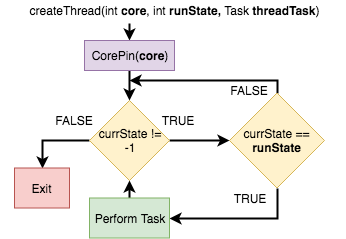
\includegraphics{Thread_Structure.png}
    \caption{Thread Flow Chart}
    \label{fig:thread-flowchart}
\end{figure}

The flowchart visualises what is essentially a while loop that runs while we are still progressing through the benchmark, and an if statement that will trigger the desired behaviour under certain global state conditions. \\
\\
The benchmarks are capable of measuring Remote L1 Load Latencies in the Modified and Exclusive states from the \texttt{MESIF} Cache Coherence Protocol(which was briefly discussed in Section \ref{sec:mesi-protocol} and Section \ref{sec:mesif-protocol}) but were not fully completed for loads to lines in the Shared state. It is  important to note that it was chosen that only 1 thread is pinned to a Core, as this will avoid the complications of assigning multiple threads to the same Core that were briefly outlined in Section \ref{knl-threading}. It was observed that filling every logical core\footnote{Logical Core: If a Core is capable of executing 4 Threads simultaneously, the OS sees this Core as 4 Logical Cores.} would increase the execution times of benchmarks, and produce incorrect results, likely as a result of the threads sharing Core resources.

\subsection{Thread Tasks}
Tasks are pinned to cores depending on the latency we want to measure. We will refer to the \emph{Base Core} as the Core where the Cache Line's of interest exists in the desired State, and the \emph{Target Core} to be the Core we wish to access said lines in the \emph{Base Core} from. For example, to measure the latency of Core 5 accessing data that exists in Core 0's L1 Cache in Modified State, the \emph{Base Core} would be Core 0, and the \emph{Target Core} would be Core 5. In the case of measuring latencies to data in the Shared state, we refer to the \emph{Alt Core} as the Core which will also hold the shared data alongside the \emph{Base Core}.

\subsubsection{Write Data}
Figure \ref{fig:write-data-task-code} shows how a thread could own Modified State data. It involves iterating over the shared data, and assigning new values to each index. Upon completing the for loop, all the data will exist in the Modified state in the L1 Cache of the Core that the thread was pinned to.
\begin{figure}[!h]
    \centering
    \begin{minipage}{0.7\textwidth}
    \begin{minted}[linenos]{cpp}
for (int i=0; i < 300; i++) {
    shared_data[i] = i;
}
currState++;
    \end{minted}
    \end{minipage}
    \caption{Write Data Task - C++ Code}
    \label{fig:write-data-task-code}
\end{figure}

\subsubsection{Read Data}
Figure \ref{fig:read-data-task-code} shows how a thread could own Exclusive/Shared data. It involves iterating over the shared data, and performing loads to the data (using the Load technique discussed in Section \ref{sec:gen-loads}). Upon completing the for loop, all the data will exist in either Exclusive or Shared state in the L1 Cache of the Core that the thread was pinned to, depending on what tasks the other threads are assigned.
\begin{figure}[!h]
    \centering
    \begin{minipage}{0.7\textwidth}
    \begin{minted}[linenos]{cpp}
for (int i=0; i < 300; i++) {
    asm volatile (
        "\n\tmov %1, %0"
        "\n\tMFENCE"
        :"=r"(shared_data[i])
        :"r"(shared_data[i]):
    );
}
currState++;
    \end{minted}
    \end{minipage}
    \caption{Read Data Task - C++ Code}
    \label{fig:read-data-task-code}
\end{figure}

\subsubsection{Time Data Access}\label{coherence-timing-task}
The thread purposed with timing the remote access uses the same method of accessing the data that was used in the previous latency benchmarks,  in Section \ref{measuring-latency}, which results in the same code used in Figure \ref{fig:timestamp_usage_l1} to time 26 Loads to different Cache Lines within the range of \texttt{shared\_data[0]} to \texttt{shared\_data[300]}. Figure \ref{fig:time-access} again shows the code snippet. The latencies measured are again stored in an array, where index \texttt{i} of the array contains the number of times a latency of \texttt{i} cycles was measured.

\begin{figure}[!h]
    \centering
    \begin{minted}[linenos]{python}
start = start_timestamp()
# Start Critical Section
# Perform 26 Loads to shared data.
load(shared_data[0])
asm("MFENCE")
load(shared_data[1])
asm("MFENCE")
...
load(shared_data[25])
asm("MFENCE")
# End Critical Section
end   = end_timestamp()

latency = (end - start - overhead) / 26
latencies[latency]++    # Increment count of this latency seen
    \end{minted}
    \caption{Pseudocode for Timing Data Accesses}
    \label{fig:time-access}
\end{figure}

\subsubsection{Dead Task}
For cores that are not in use, there is a "Dead Task" which simply stalls until the \texttt{currState} is set to -1 (marking the experiment is over), then the thread returns/exits. These dead tasks are allocated to cores to ensure that each core has an active running thread, to ensure that all Core's are active.

\subsection{Remote L1 Modified Read}
\subsubsection{Thread/Task Allocation}
To perform a load to a Modified Cache Line in a Remote L1 Cache, we must have our Base Core modify the data, and then our Target Core should perform the timed accesses to the data that is in the Modified State. Using the Flow Chart in Figure \ref{fig:thread-flowchart} as our \texttt{createThread()} method, we can use the following pseudocode to generate our benchmark:

\begin{figure}[!h]
    \centering
    \begin{minipage}{0.7\textwidth}
    \begin{minted}[linenos]{cpp}
currState = 0
// Set Write Task on State 1
createThread(BASE_CORE, 1, write)
// Set Timing Task on State 2
createThread(TARGET_CORE, 2, time_access)
/* Assign Dead Tasks to all other Cores */
for (int i=0; i < NUM_CORES; i++) {
    if (i != BASE_CORE && i != TARGET_CORE)
        createThread(i, -1, dead_task)
}
/* Set State to 1 to get Tasks Started */
currState = 1
while (currState != 3) { /* Spin */ }
/*Set State to -1 to end all Threads/Tasks */
currState = -1
    \end{minted}
    \end{minipage}
    \caption{Remote Modified Read - Thread/Task Allocation Pseudocode}
    \label{fig:remote-M-read-pseudo}
\end{figure}

\newpage
\subsubsection{State Diagram}
\begin{figure}[!h]
    \centering
    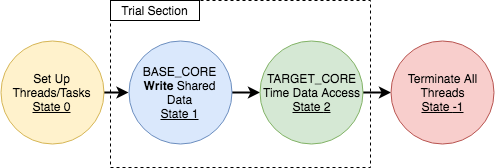
\includegraphics[width=100mm]{ModifiedState.png}
    \caption{Remote L1 Modified Read State Machine}
    \label{fig:remote-M-read-state}
\end{figure}

\subsubsection{Summary}
In summary, to obtain a latency measurement for a load to a Modified Line in a remote L1 Cache, there must be a Core which performs \textbf{writes} to a set of shared data, and in turn, sets it to Modified state in the Cores local Cache. Then, another Core must attempt to read the same set of shared data, which will incur a local Cache miss, and the data will be fetched from the \emph{Base Core} which owns the data in Modified State. The key features outlined in Section \ref{sec:l1-lat-key-comp}, \ref{sec:l2-lat-key-comp}, and \ref{sec:mem-lat-key-comp} all apply including the \textit{Data Declaration Consideration} outlined in Section \ref{data-declaration-consideration-L2}, which has minor modifications in implementation to ensure the same global and shared variable can be used independently and uniquely within the \textit{Trial Section} outlined in Figure \ref{fig:remote-M-read-state}. The repeated trials are performed by the following code snippet as a drop-in replacement for Lines 12 to 15 in Figure \ref{fig:remote-M-read-pseudo}:
\begin{figure}[!h]
    \centering
    \begin{minipage}{0.8\textwidth}
    \begin{minted}[linenos]{cpp}

for (int i = 0; i < 1000; i++) {    // Do 1000 Trials.
    currTask = 0;
    // Re-allocate shared data to invalidate across all Cores.
    shared_data = (int*)malloc(L2_SIZE_B);
    currTask = 1;

    /* Threads Complete their Tasks */
        
    while (currTask != 3) { /* Wait for all 2 Tasks to complete. */ }
    
    // Delete our shared data to prevent memory leaks.
    delete shared_data;
}
currTask = -1;  // Signal threads to terminate.
    \end{minted}
    \end{minipage}
    \caption{Remote Modified Read - Repeated Trials}
    \label{fig:remote-M-repeat}
\end{figure}


\subsection{Remote L1 Exclusive Read}
\subsubsection{Thread/Task Allocation}
To perform a load to a Cache Line in the Exclusive state in a Remote L1 Cache, we must have our Base Core load the data, and then our Target Core should perform the timed accesses to the data in the Exclusive State. Again, using the Flow Chart in Figure \ref{fig:thread-flowchart} as our \texttt{createThread()} method, we can use the following pseudocode to generate our benchmark:

\begin{figure}[!h]
    \centering
    \begin{minipage}{0.7\textwidth}
    \begin{minted}[linenos]{cpp}
currState = 0

// Set Read Task on State 1 on Core BASE_CORE
createThread(BASE_CORE, 1, read)
// Set Timing Task on State 2 on Core TARGET_CORE
createThread(TARGET_CORE, 2, time_access)
/* Assign Dead Tasks to all other Cores */
for (int i=0; i < NUM_CORES; i++) {
    if (i != BASE_CORE && i != TARGET_CORE)
        createThread(i, -1, dead_task)
}
/* Set State to 1 to get Tasks Started */
currState = 1
while (currState != 3) { /* Spin */ }
/*Set State to -1 to end all Threads/Tasks */
currState = -1
    \end{minted}
    \end{minipage}
    \caption{Remote Exclusive Read - Thread/Task Allocation Pseudocode}
    \label{fig:remote-E-read-pseudo}
\end{figure}

\newpage
\subsubsection{State Diagram}
\begin{figure}[!h]
    \centering
    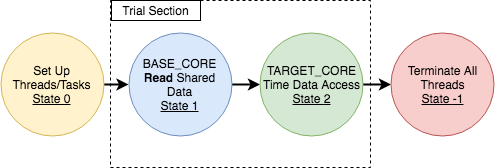
\includegraphics[width=100mm]{ExclusiveState.png}
    \caption{Remote L1 Exclusive Read State Machine}
    \label{fig:remote-E-read-state}
\end{figure}

\subsubsection{Summary}
In summary, to obtain a latency measurement for a load to an Exclusive Line in a remote L1 Cache, there must be a Core which performs \textbf{loads} to a set of shared data, and in turn, sets it to Exclusive state in the Cores local Cache. Then, another Core must attempt to read the same set of shared data, which will incur a local Cache miss, and the data will be fetched from the \emph{Base Core} which owns the data in the Exclusive State. The key features outlined in Section \ref{sec:l1-lat-key-comp}, \ref{sec:l2-lat-key-comp}, and \ref{sec:mem-lat-key-comp} all apply including the \textit{Data Declaration Consideration} outlined in Section \ref{data-declaration-consideration-L2}, which has minor modifications in implementation to ensure the same global and shared variable can be used independently within the \textit{Trial Section} outlined in Figure \ref{fig:remote-M-read-state}. The repeated trials are performed by the following code snippet as a drop-in replacement for Lines 13 to 16 in Figure \ref{fig:remote-E-read-pseudo}:
\begin{figure}[!h]
    \centering
    \begin{minipage}{0.8\textwidth}
    \begin{minted}[linenos]{cpp}
// Do 1000 Trials.
for (int i = 0; i < 1000; i++) {
    currTask = 0;
    // Re-allocate shared data to invalidate across all Cores.
    shared_data = (int*)malloc(L2_SIZE_B);
    currTask = 1;

    /* Threads Complete their Tasks */
        
    while (currTask != 3) {
        /* Wait for all 2 Tasks to complete. */
    }

    // Delete our shared data to prevent memory leaks.
    delete shared_data;
}
currTask = -1;  // Signal threads to terminate.
    \end{minted}
    \end{minipage}
    \caption{Remote Exclusive Read - Repeated Trials}
    \label{fig:remote-E-repeat}
\end{figure}

\subsection{Remote L1 Shared Read}\label{sec:shared-read}
\subsubsection{Thread/Task Allocation}
To perform a Remote L1 Read to Shared Cache Lines, we must have our \emph{Base Core} read the shared data, then have another Core (our \emph{Alt Core}) read the same shared data, and then finally our Target Core should perform the timed accesses to the shared lines in the Shared State. This scenario is a little more complex than the previous two, as it involves the use of a third Core, which makes the benchmark more complex. It is more complex because we cannot definitively say if it will be the \emph{Base Core} or the \emph{Alt Core} that will own the lines in the \textit{Forward State}/\textit{Shared State}, meaning that we must take care when deciding which Cores to use. Again, using the Flow Chart in Figure \ref{fig:thread-flowchart} as our \texttt{createThread()} method, we can use the following pseudocode to generate our Benchmark:

\begin{figure}[!h]
    \centering
    \begin{minipage}{0.7\textwidth}
    \begin{minted}[linenos]{cpp}
currState = 0
// Set Read Task on State 1
createThread(BASE_CORE, 1, read)
// Set Read Task on State 2
createThread(ALT_CORE, 2, read)
// Set Timing Task on State 3
createThread(TARGET_CORE, 3, time_access)
/* Assign Dead Tasks to all other Cores */
for (int i=0; i < NUM_CORES; i++) {
    if (i != BASE_CORE && i != TARGET_CORE && i != ALT_CORE)
        createThread(i, -1, dead_task)
}
/* Set State to 1 to get Tasks Started */
currState = 1
while (currState != 4) { /* Spin */ }
/*Set State to -1 to end all Threads/Tasks */
currState = -1
    \end{minted}
    \end{minipage}
    \caption{Remote Shared Read - Thread/Task Allocation Pseudocode}
    \label{fig:remote-S-read-pseudo}
\end{figure}


\subsubsection{State Diagram}
\begin{figure}[!h]
    \centering
    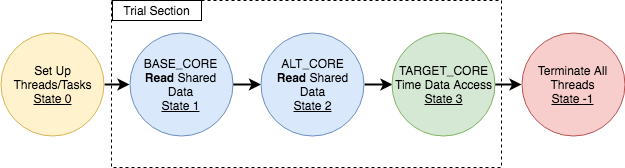
\includegraphics[width=125mm]{SharedState.png}
    \caption{Remote L1 Shared Read State Machine}
    \label{fig:remote-S-read-state}
\end{figure}

\subsubsection{Summary}
In summary, to obtain a latency measurement for a load to a Shared Line in a remote L1 Cache, there must be a Core which performs \textbf{loads} to a set of shared data, and in turn, sets it to Exclusive state in that Cores local Cache. Then, another Core must perform the same set of \textbf{loads}, which will miss in the Core's Local Cache, and the Cache Lines will be retrieved from a Remote Core (the \emph{Base Core}), and the State of those Cache Lines will be updated to Shared State in both Cores. Finally, another Core must attempt to load the same set of shared data, which will incur a local Cache miss, and the data will be fetched from the Core that owns the Cache Lines in the \textit{Forward State}. As with the Modified/Exclusive benchmarks, the key features outlined in Section \ref{sec:l1-lat-key-comp}, \ref{sec:l2-lat-key-comp}, and \ref{sec:mem-lat-key-comp} all still apply, including the Data Declaration Consideration outlined in Section \ref{data-declaration-consideration-L2}. The repeated trials are performed by the following code snippet:
\begin{figure}[!h]
    \centering
    \begin{minipage}{0.8\textwidth}
    \begin{minted}[linenos]{cpp}
// Do 1000 Trials.
for (int i = 0; i < 1000; i++) {
    currTask = 0;
    // Re-allocate shared data to invalidate across all Cores.
    shared_data = (int*)malloc(L2_SIZE_B);
    currTask = 1;

    /* Threads Complete their Tasks */
        
    while (currTask != 4) {
        /* Wait for all 3 Tasks to complete. */
    }

    // Delete our shared data to prevent memory leaks.
    delete shared_data;
}
currTask = -1;  // Signal threads to terminate.
    \end{minted}
    \end{minipage}
    \caption{Remote Shared Read - Repeated Trials}
    \label{fig:remote-S-repeat}
\end{figure}

\newpage


\section{DRAM/MCDRAM Bandwidth}\label{mcdram-dram-benchmarks-bw}
\subsection{STREAM Benchmark}
The STREAM Benchmark is designed for evaluating High Performance Computing (HPC) systems. HPC systems typically work with large data sets that cannot fit within a typical Cache system. Data of this nature means that processors are typically spending a lot of time waiting for data to be transferred to-and-from memory systems such as DRAM or MCDRAM, and the STREAM benchmark evaluates how much data chips such as the KNL can process per second. In order to evaluate the performance of a chip in an HPC context, the STREAM benchmark tests four "kernels", which are essentially memory and CPU intensive operations that are common in HPC applications.

\begin{table}[!h]
\begin{center}
\caption{STREAM Kernels}
\label{fig:stream-kernels}
\begin{tabular}{ |c|c| } 
    \hline
    Kernel Name & Kernel Operation(s) \\
    \hline\hline
    COPY    & \texttt{a(i) = b(i)} \\
    \hline
    SCALE   & \texttt{a(i) = q*b(i)} \\
    \hline
    SUM     & \texttt{a(i) = b(i) + c(i)} \\
    \hline
    TRIAD   & \texttt{a(i) = b(i) + q*c(i)} \\
    \hline
\end{tabular}
\end{center}
\end{table}

Table \ref{fig:stream-kernels} shows the different kernels operations. As we can see, the \texttt{COPY} Kernel copies data from one memory location to another. The \texttt{SCALE} kernel scales up all data in a region by a certain coefficient. The \texttt{SUM} kernel sums data from two sources and stores in a third. Finally, the \texttt{TRIAD} performs an amalgamation of all the previous kernels.

\subsection{STREAM Usage}
It is important to ensure that when performing STREAM benchmarks, we perform the benchmarks using the guidelines provided.
\subsubsection{Compilation}
Compilation of the STREAM benchmark is important in ensuring that the benchmark can be run in a parallel fashion properly. As such the code was compiled using the following command:
\begin{center}
    \texttt{cc stream.c -O3 -o stream -fopenmp -DSTREAM\_ARRAY\_SIZE=64000000}
\end{center}
It is important to include the \texttt{-fopenmp} flag, as this will ensure that the code that is marked with \texttt{"\#pragma omp parallel for"} will be parallelised appropriately. We also define the \texttt{STREAM\_ARRAY\_SIZE} to be sufficiently large in accordance with the guidelines.

\subsubsection{Running}
In order to run the STREAM benchmark in a reliable parallel fashion, it must be invoked by a run-script that exports appropriate environment variables.
{
\begin{figure}[!h]
    \centering
    \begin{minted}[linenos]{bash}
export OMP_PROC_BIND=true
OMP_NUM_THREADS=1   numactl --membind 0 ./stream 
    \end{minted}
    \caption{Sample of STREAM Run Script}
    \label{fig:stream-run-script}
\end{figure}
} \\

Figure \ref{fig:stream-run-script} shows a sample of the \texttt{run.sh} script used to invoke the STREAM benchmark. Line 1 exports an environment variable which will ensure that OpenMP Threads cannot be migrated between Cores. Then \texttt{"OMP\_NUM\_THREADS=1"} specifies that there should be exactly 1 OpenMP Thread created. The full run script rials with different numbers of OpenMP Threads, scaling exponentially from 1 Thread to 128 Threads. The \texttt{"numactl --membind 0"} call ensures that the program is run on the appropriate NUMA region. Although the memory location here is bound to NUMA Region 0, this value is substituted with the parameter of the run script, such that different NUMA Regions can be tested.

\newpage

\chapter{Results}\label{chap:results}
Results were obtained on a 64 Core Intel Xeon Phi CPU 7210 Clocked at 1.30GHz.
\section{Latencies}

\subsection{Intra-Tile Latencies}
Intra-Tile Latencies are Latencies of accessing data in Modified/Exclusive State. In the context of these results, \textbf{Local} refers to the same Core, and \textbf{Remote} refers to the other \emph{Core} that is on the same \emph{Tile}.
\begin{table}[!h]
\begin{center}
\caption{Intra-Tile Latencies}
\label{fig:intra-tile-latencies}
\begin{tabular}{ |c|c| } 
    \hline
    Cache & Latency \\
    \hline
    Local L1 Cache & 0.77ns (1 Cycle) \\
    Local L2 Cache & 5.38ns (7 Cycles) \\
    Remote L1 Cache[M/E] & 11.54ns (15 Cycles) \\
    \hline
\end{tabular}
\end{center}
\end{table}

\subsection{Inter-Tile Latencies}
 Inter-Tile Latencies are the Latencies of accessing data in other Tile's L1 Cache in Modified/Exclusive State. In the context of these results, \textbf{Local} refers to the same \emph{NUMA Region}, and \textbf{Remote} refers to another \emph{NUMA Region}.
\begin{table}[!h]
\begin{center}
\caption{Inter-Tile Latencies}
\label{fig:inter-tile-latencies}
\begin{tabular}{ |c|c|c| } 
    \hline
    L2 Cache Config & Latency \\
    \hline
    All-to-All & 26.15ns (34 Cycle) \\
    Quadrant & 26.15ns (34 Cycle) \\
    Sub NUMA Local & 25.38ns (33 Cycle) \\
    Sub NUMA Remote & 27.69ns (36 Cycle) \\
    \hline
\end{tabular}
\end{center}
\end{table}

\newpage
\subsection{MCDRAM/DRAM Latencies}
MCDRAM/DRAM Latencies are the Latencies of accessing data that exists only in DRAM or MCDRAM. In the context of these results, \textbf{Local} refers to the memory in the same \emph{NUMA Region}, and \textbf{Remote} refers to memory in another \emph{NUMA Region}.
\begin{table}[!h]
\begin{center}
\caption{MCDRAM Latencies}
\label{fig:mcdram-latencies}
\begin{tabular}{ |c|c|c|c| } 
    \hline
    L2 Cache Config & Memory Config & Latency \\
    \hline
    All-to-All      & Flat  & 169.23ns (220 Cycles) \\
    All-to-All      & Cache & 169.23ns (220 Cycles) \\
    Quadrant        & Flat  & 165.38ns (215 Cycles) \\
    Quadrant        & Cache & 165.38ns (215 Cycles) \\
    Sub NUMA Local  & Flat  & 161.54ns (210 Cycles) \\
    Sub NUMA Local  & Cache & 161.54ns (210 Cycles) \\ % eeeh
    Sub NUMA Remote & Flat  & 173.85ns (226 Cycles) \\
    Sub NUMA Remote & Cache & 173.85ns (226 Cycles) \\
    \hline
\end{tabular}
\end{center}
\end{table}

\begin{table}[!h]
\begin{center}
\caption{DRAM Latencies}
\label{fig:dram-latencies}
\begin{tabular}{ |c|c|c|c| } 
    \hline
    L2 Cache Config & Memory Config & Latency \\
    \hline
    All-to-All      & Flat  & 134.62ns (175 Cycles) \\
    Quadrant        & Flat  & 133.08ns (173 Cycles) \\
    Sub NUMA Local  & Flat  & 127.69ns (166 Cycles) \\
    Sub NUMA Remote & Flat  & 138.46ns (180 Cycles) \\
    \hline
\end{tabular}
\end{center}
\end{table}


\newpage

\section{Bandwidths}

\subsection{All-to-All}

\begin{figure}[!h]
    \centering
    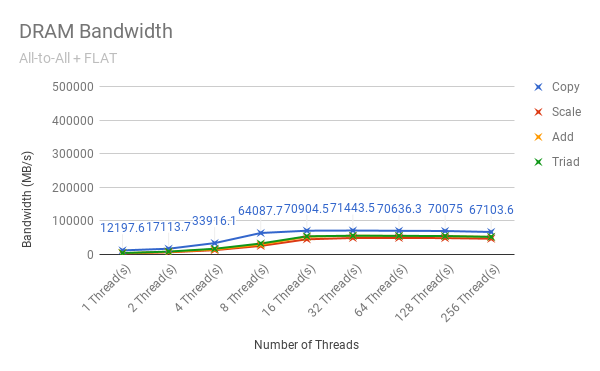
\includegraphics[width=\textwidth]{Results/dram_a2a_f.png}
    \caption{DRAM - Flat Mode}
    \label{res:dram-a2a-f}
\end{figure}

\begin{figure}[!h]
    \centering
    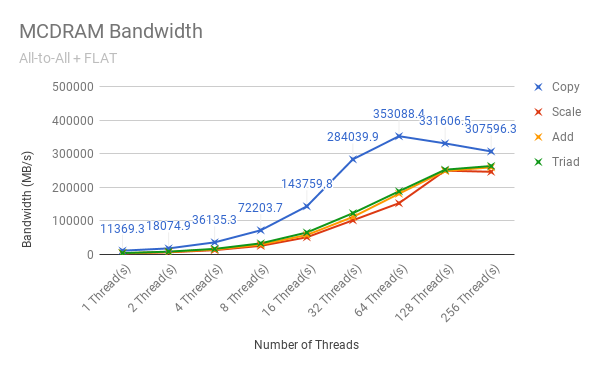
\includegraphics[width=\textwidth]{Results/mcdram_a2a_f.png}
    \caption{MCDRAM - Flat Mode}
    \label{res:mcdram-a2a-f}
\end{figure}

\begin{figure}[!h]
    \centering
    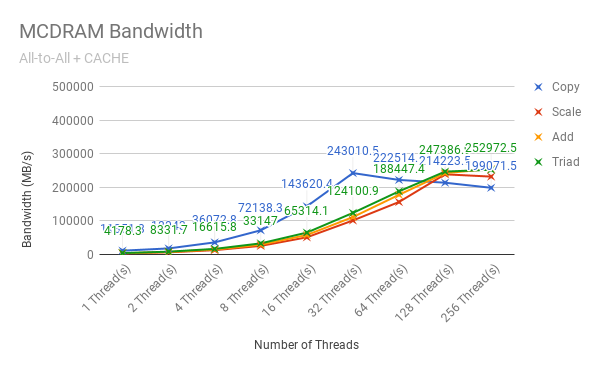
\includegraphics[width=\textwidth]{Results/mcdram_a2a_c.png}
    \caption{MCDRAM - Cache Mode}
    \label{res:mcdram-a2a-c}
\end{figure}

\newpage
\newpage

\subsection{Quadrant}

\begin{figure}[!h]
    \centering
    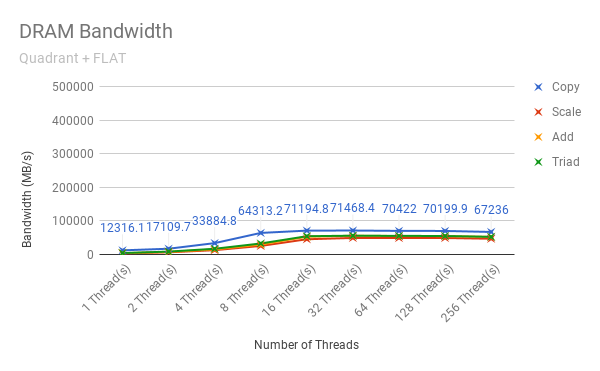
\includegraphics[width=\textwidth]{Results/dram_quad_f.png}
    \caption{DRAM - Flat Mode}
    \label{res:dram-quad-f}
\end{figure}

\begin{figure}[!h]
    \centering
    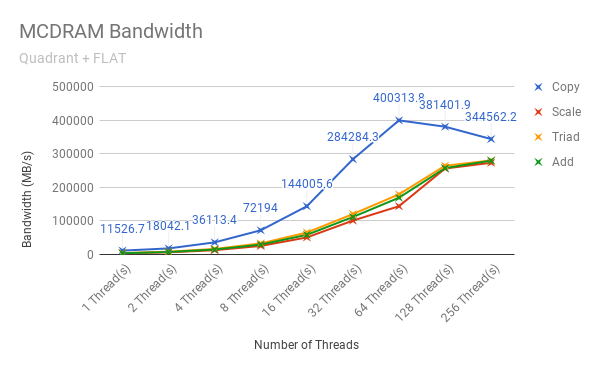
\includegraphics[width=\textwidth]{Results/mcdram_quad_f.png}
    \caption{MCDRAM - Flat Mode}
    \label{res:mcdram-quad-f}
\end{figure}

\begin{figure}[!h]
    \centering
    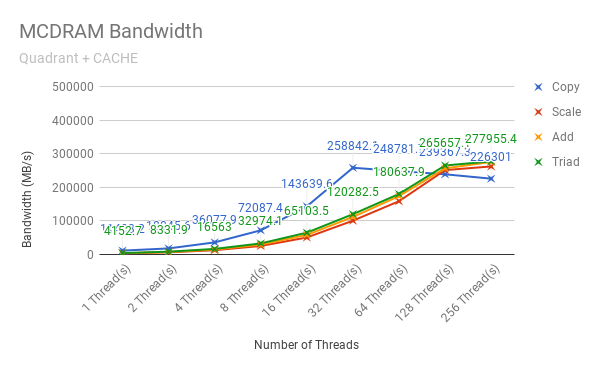
\includegraphics[width=\textwidth]{Results/mcdram_quad_c.png}
    \caption{MCDRAM - Cache Mode}
    \label{res:mcdram-quad-c}
\end{figure}

\newpage

\subsection{Sub-NUMA}

\begin{figure}[!h]
    \centering
    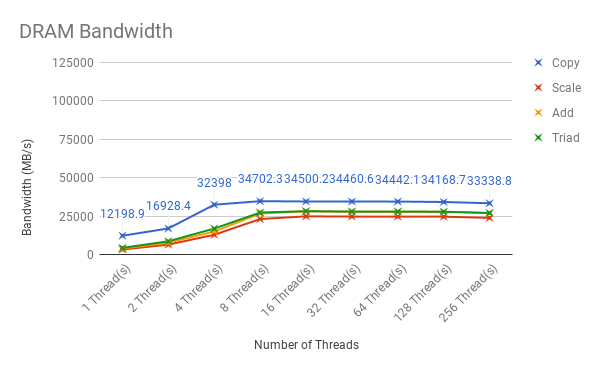
\includegraphics[width=\textwidth]{Results/dram_snc4_f.png}
    \caption{DRAM - Flat Mode}
    \label{res:dram-snc4-f}
\end{figure}

\begin{figure}[!h]
    \centering
    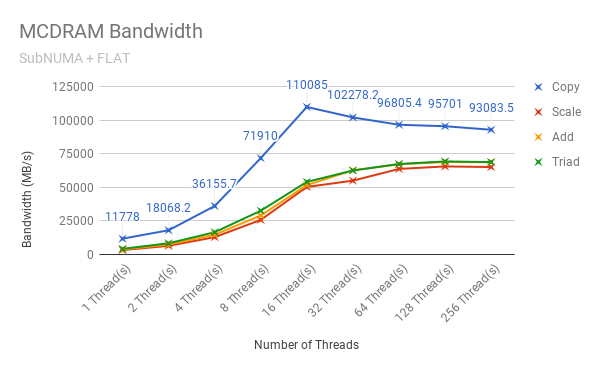
\includegraphics[width=\textwidth]{Results/mcdram_snc4_f.png}
    \caption{MCDRAM - Flat Mode}
    \label{res:mcdram-snc4-f}
\end{figure}

\begin{figure}[!h]
    \centering
    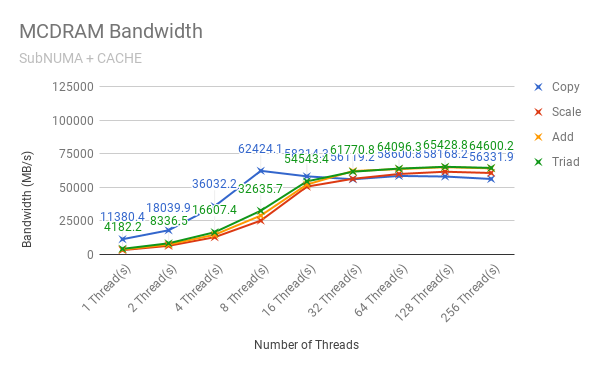
\includegraphics[width=\textwidth]{Results/mcdram_snc4_c.png}
    \caption{MCDRAM - Cache Mode}
    \label{res:mcdram-snc4-c}
\end{figure}

\chapter{Discussion}\label{chap:discussion}
When discussing results, I will refer to the system presented in the paper by Hackenberg, Molka and Nagel\cite{cache-coherence-paper} as the "Nehalem" system.
\section{Latency Conclusions}
\subsection{Intra-Tile Results}
\subsubsection{Local L1 Cache}
The measured Latencies in Table \ref{fig:intra-tile-latencies} follow an expected trend. We see that an L2 Access takes longer than an L1 Access, and that Accessing data in the Tile's adjacent Core L1 takes roughly twice the time of an L2 Access. However, it is possible that the results could be incorrect. If we refer to the Nehalem system, we see that their test system is a 2.6GHz Chip with a measured L1 Latency of 1.3ns/4 Cycles. Our benchmarks were run on a 1.3GHz chip and resulted in 0.77ns/1 Cycle. It is unlikely that Intel (roughly) halved the latency of an L1 Cache access, and is it more likely that there is some error within the timing mechanism that could cause incorrect rounding of Cycles when measuring multiple loads. If we consider an Intel article published by Eric G.\cite{eric-intel-article}, it specifies that the L1 Data Cache has two 64B Load Ports. Despite including Memory Fences after every load, it could be possible that the underlying architecture is able to process 2 Loads simultaneously. If it were the case that our microbenchmark loads were processed two at a time, then our measured latency would, in fact, be roughly double the observed. This would make our L1 Latency be 1.54ns, which aligns more with observed Latencies on other Intel architectures. Had more time been available, more work could have been done to deeper investigate how the number of loads timed would affect the measured latency.

\subsubsection{Local L2 Cache}
The Local L2 Cache Latency measured (Table \ref{fig:intra-tile-latencies}) was 5.38ns/7 Cycles. This seems like a reasonable value for an L2 Latency, and when comparing to the Nehalem system, we see that that the Nehalem system had a measured Local L2 Cache Latency is 3.4ns/10 Cycles. Given that the Nehalem system's L2 Cache is 256KB, and our test system's L2 Cache is 1024KB, it would be feasible for the Latency of accessing our system's larger L2 Cache to be higher. Similar to the L1 Cache, it could be possible for the L2 Cache to be dual-ported, and therefore could be processing two loads simultaneously. More work could be done to verify the integrity of the results for example by performing benchmarks on a range of loads. Error may also have been introduced due to the methodology for generating L1 Misses/L2 Hits, perhaps investigating methodologies of properly thrashing\footnote{Thrashing the L1 Cache: Putting the L1 Cache under intense usage, in order to thoroughly remove all existing entries.} the L1 Cache with dead data would have provided more reliable results.

\subsubsection{Remote L1 Cache}
The measured Latency for a Remote L1 Cache on a Tile was 11.54ns/15 Cycles. \\

\begin{figure}[!h]
    \centering
    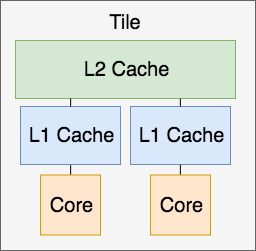
\includegraphics[width=5cm]{Tile.png}
    \caption{Tile Memory Pictorial}
    \label{fig:tile-memory}
\end{figure}
If we consider Figure \ref{fig:tile-memory} to be the architecture of the memory system within a Tile, it would make sense that our measured Latency would be 15 Cycles. If we consider that it would take 7 Cycles to determine if the Line exists in the L2, it would then make sense for another ~7 Cycles to retrieve data from the remote L1 Cache, and deliver it to the consuming Core. However as we have already discussed the possible issues that could prevent accurate measurements, we must also consider that similar issues could be carried over into or made more complex in this microbenchmark.

\subsection{Inter-Tile Results}
Unfortunately, results for accessing data in the Shared state were not reliably measured due to inconsistent and bizarre measured latencies. This may have been due to a lack of understanding of how the MESIF Protocol works, and lack of a deterministic way of determining which Core would be assigned the \emph{Forward} state. When considering the Modified/Exclusive Latencies, in the respective L2 Modes, measured Modified and Exclusive latencies were identical, and are shown in Table \ref{fig:inter-tile-latencies} as a single Latency. There definitely exists an error in the results, as we would expect the latency of accessing remote data in Quadrant mode would be lower than the latency of accessing remote data in All-to-All as per Intel's Presentation on KNL\cite{intel_pres}. However, an encouraging trend shows that accessing remote data in a Local Sub-NUMA configuration is faster than all other Cache configurations. It should also be expected that accessing data in a remote NUMA region would incur a large latency, as in theory, it should involve an access to main memory in the fashion detailed in Section \ref{snc4-explained}(Under \textit{Sub-NUMA Clustering}). Given that the measured latency for accessing data in a remote NUMA region was 27.69ns/36 Cycles, it is safe to say that an error exists in the experiment/methodology. When conducting the experiments, I ran the programs using the \texttt{numactl} program, ensuring that the NUMA region the program was loaded into was chosen appropriately for measuring remote accesses, verifying that tasks were pinned to appropriate Core using the output of calling \texttt{numactl -H}\footnote{\texttt{numactl -H}: Lists all NUMA regions in the system, and which cores exist in which regions.}. Pinning Tasks to Cores on the same Tile does drastically reduce the Latency(see "Remote L1 Cache" in Table \ref{fig:intra-tile-latencies}) which indicates that the results are somewhat correct, however, I suspect that perhaps thread placement was not performed properly with respect to the NUMA regions, and had more time been available, research into how to validate this could have highlighted potential issues or verified existing results. In conclusion, I do not believe the results to be reliable, but the consistency of the results and the general trends indicate that there is a solid foundation for microbenchmarking cache coherence latencies.

\subsection{MCDRAM/DRAM Latencies Results}
When conducting MCDRAM/DRAM Latencies, care was taken to ensure that the Latencies measured were accesses to data on a single NUMA Node, to avoid the Latencies of cross-NUMA accesses. \\
\\
John McCalpin has conducted microbenchmarks to measure the latencies of the MCDRAM and DRAM in different L2 Cache/Memory Configurations\cite{mccalpin_results}. This is useful as it allows us to compare the results obtained for correctness, which can, in turn, validate aspects of our benchmark suite. \\
\\
As can be seen in Table \ref{fig:mcdram-latencies}, the Memory Configuration has no effect on Latency. The following relationship on access latencies holds for both MCDRAM and DRAM:
\begin{equation}\label{dram-latency-relationship}
\textrm{Sub-NUMA Local} \leq \textrm{Quadrant} \leq \textrm{All-to-All} \leq \textrm{Sub-NUMA Remote}
\end{equation}
Equation \ref{dram-latency-relationship} shows an observed trend that we would expect to see in our results. Furthermore, we can compare our results to those obtained by John McCalpin, and we see the following similarities/differences:

\begin{table}[!h]
\begin{center}
\caption{\textbf{DRAM} Latencies Verification (Flat Mode)}
\label{fig:dram-latencies-verification}
\begin{tabular}{ |c|c|c| } 
    \hline
    L2 Cache Config & McCalpin's Average Latency & Our Average Latency \\
    \hline
    All-to-All      & 131.8ns  & 134.62ns \\
    Quadrant        & 130.4ns  & 133.08ns \\
    Sub NUMA Local  & 128.2ns  & 127.69ns \\
    Sub NUMA Remote & 133.1ns  & 138.46ns \\
    \hline
\end{tabular}
\end{center}
\end{table}

\begin{table}[!h]
\begin{center}
\caption{\textbf{MCDRAM} Latencies Verification (Flat Mode)}
\label{fig:mcdram-latencies-verification}
\begin{tabular}{ |c|c|c| } 
    \hline
    L2 Cache Config  & McCalpin's Average Latency & Our Average Latency \\
    \hline
    All-to-All      & 155.9ns  & 169.23ns \\
    Quadrant        & 154.0ns  & 165.38ns \\
    Sub NUMA Local  & 150.5ns  & 161.54ns \\
    Sub NUMA Remote & 156.8ns  & 173.85ns \\
    \hline
\end{tabular}
\end{center}
\end{table}

Table \ref{fig:dram-latencies-verification} shows a comparison of our measured DRAM Latencies with John McCalpin's. The comparison shows that although our results are not identical (which is to be expected when dealing with DRAM), we follow a close trend. This trend can be seen if we look at the latency difference between different L2 Cache Configs; for example, the difference in latency between All-to-All and Quadrant was roughly 1.4ns in our measurements, and McCalpins. Similar observations can be made when comparing other modes, but with larger margins of error. This property again indicates that our microbenchmarks follow a correct design, but errors exist. I would hypothesise that some error exists within the timing mechanism, due to this trend of slights inconsistencies that exist among all latency benchmarks. Looking at Table \ref{fig:mcdram-latencies-verification} also aligns with this hypothesis, as we see more examples of relative trends.


\section{MCDRAM/DRAM Bandwidth Results}
Figures \ref{res:dram-a2a-f} through \ref{res:mcdram-snc4-c} show the results of the STREAM\cite{STREAM} Benchmark under the conditions mentioned in Section \ref{mcdram-dram-benchmarks-bw}. Across all the benchmarks, we can see that the peak bandwidth measured using MCDRAM is in Figure \ref{res:mcdram-quad-f}, with a peak bandwidth of ~400GB/s, similarly, the peak DRAM bandwidth measured is in Figure \ref{res:dram-quad-f} (or alternatively at a scaled resolution, in Figure \ref{res:dram-quad-f-scaled}), with a peak bandwidth of ~70.5GB/s. Intel declared\cite{intel_pres} that peak bandwidth for DRAM memory would be 90+ GB/s and peak bandwidth for MCDRAM memory would be 400+ GB/s under the STREAM's Triad 'operation'. Comparing to our peak results we see that we are able to achieve 400GB/s for MCDRAM, but only 70GB/s for DRAM under a Copy operation. There are two major observations here. Firstly; peak bandwidths were observed under the Copy operation, and Secondly; our peak bandwidths are slightly lower than those declared by Intel. Both of these observations are likely due to our test system being a 64 Core system, where there exists a Knights Landing model that contains 72 Cores. It is reasonable to believe that a 72 Core system would be able to obtain higher bandwidths, considering that more threads could be run simultaneously. That said, our measured bandwidths closely follow the expected trend; MCDRAM has \texttt{4x} the bandwidth of DRAM. Another trend in the results that is noteworthy, is we see the bandwidth increase up until 64 Threads, where we see the bandwidth either plateau or drop off. This makes sense, as our test system has 64 Cores, and there is an expected performance hit when multiple threads are running on a Core concurrently, sharing the Core's resources. We also see that in the case of Sub-NUMA Clustering, our peak measured bandwidths are roughly one-quarter of the peak measured bandwidth in \texttt{Quadrant} mode, which is the expected behaviour.

\section{Summary}
To summarise the results, it would be fair to say that the declared Bandwidths provided by Intel are accurate, and that bandwidths measured on our 64 Core test system would not achieve peak bandwidths relative to the 72 Core Knights Landing chips. When measuring latencies, it appears that the timing mechanism proposed by Intel\cite{code_exec_times} does provide a reliable timing mechanism for measuring code execution times, but perhaps loses accuracy when measuring load instructions. Had more time been available, further experimenting with the number of loads, or experimenting other memory access approaches could have been tried. For example, pointer chasing\footnote{Pointer Chasing: Traversing a linked list, in order to achieve unpredictable memory accesses.} is a common practice in benchmarking suites for generating random accesses to memory. When creating multi-threaded benchmarks for measuring coherence latencies, more work could have been done to ensure thread placement with respect to NUMA regions was resulting in the intended behaviour. This is especially important when considering data in the Shared state, which unfortunately provided no meaningful results following the benchmark structure outlined in Section \ref{coherence-latencies} and Section \ref{sec:shared-read}.

\chapter{Conclusion}\label{chap:conclusion}
\section{Work Done}
All code and algorithms presented within this report were my own work, with the exception of the STREAM benchmark, or other code snippets which were otherwise cited. The project work began with trying many different sample programs in order to confirm my understanding of computer architecture thus far. A large portion of the work that was done was into researching, trying, and evaluating possible options for measuring latency (as discussed in Section \ref{measuring-latency}). After some base timing mechanism was established, I then worked on building algorithms to place data in specific areas of the memory hierarchy, and using the results and observations made, improvements were made to both the algorithms and the timing techniques. After obtaining measurements for all non-coherence related latencies, I primarily worked on researching how it is possible to measure the bandwidth of the DRAM/MCDRAM and reading Intel documentation on the subject. Many sources pointed to work conducted by John McCalpin, and I then worked on properly using the STREAM benchmark. The final chunk of work was looking into how to write multithreaded applications in the context of OpenMP but also simply c++ threading for the purpose of measuring Cache Coherence latencies. Due to the nature of the benchmark, it was important to have tightly synchronised threads, and so an OpenMP approach would be complicating the matter more than necessary. Using c++ threads, I worked on implementing an algorithm/program structure that would allow me to have multiple threads follow a single state machine. I then used work from my previous latency benchmarks to have threads/Cores perform actions on shared data such as reads/writes. Other work that was attempted but not fully explored includes techniques such as intentional cache thrashing to evict data from different caches, however, it did not provide immediate value to all the benchmarks written so it was not fully implemented. I also looked into using a pointer-chasing algorithm for generating random loads, but opted to try a different approach to measuring latencies relative to other benchmark programs. 

\section{Insight Gained}
Throughout working on the project, I gained a lot of insight into how computer architecture is applied in a parallel fashion under the context of High Performance Computing. For example how HPC systems processor architecture is relevant to the data processed. The project also supplied a great opportunity to confirm my prior knowledge, for example how applications are executed from a high-level, down to a very low level. An example of this is that a lot of the work included inspecting assembly and understanding how compilers generate machine code, and how code is executed. I would also say that the project introduced me to some concepts of code optimisation, for example on the importance of writing cache-friendly code. Finally, the project also provided a great opportunity to solidify my understanding of concepts taught (specifically Cache Coherence) in the Parallel Architectures course taught by Vijay Nagarajan.

\section{Project Outcome}
The outcome of the project presents a set of results for latencies and bandwidths of accessing data between different memory components of the Knights Landing processor. It is important to read the discussion of the results, as there is further room for improving the benchmark to obtain more accurate results. The project also delivers open-source benchmark programs that can be used for further research in the field. Had more time been available, further work into researching different ways of measuring latencies, and improvements on the current technique would be done. It would also be worth investigating cache thrashing, as an opportunity for placing data in specific areas of the Cache hierarchy.

\chapter{Open-Source Benchmark Suite}\label{chap:benchmark-suite}
This Chapter provides no further discussion or evaluation of the work done in this project, but shows an outline of the benchmark produced. Specifically, this chapter will introduce how one could run the benchmarks for themselves. The same instructions, plus more background info, can be found at the GitHub repository root: \\
https://github.com/acwilson96/MicroBenchmarking-KNL
\section{Repository Structure}

\begin{figure}[!h]
    \centering
    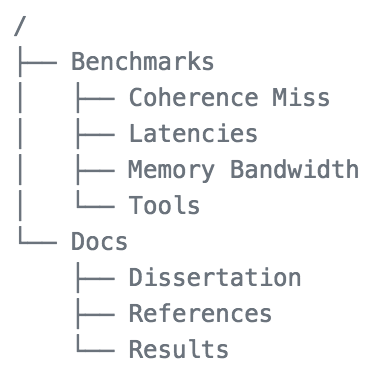
\includegraphics{Results/dir_structure.png}
    \caption{Repository Structure}
    \label{fig:repo-struct}
\end{figure}


\section{Benchmarks}
Contains source-code and associated files for building and executing the different microbenchmarks.

\subsection{Coherence Miss}
Contains source-code for the multi-threaded benchmark which evaluates latencies of accessing data across Cores. \\
\\
\textbf{Usage:}
\begin{minted}{bash}
make
./run.sh State1Core ( M | E ) State2Core
./run.sh State1Core State2Core S State3Core
\end{minted}

For example, if you wish to trial Core 5 accessing modified data in Core 8's L1 Cache, you would run \texttt{./run.sh 8 M 5}. Or if you wish for Core 1 to access Exclusive data in Core 0: \texttt{./run.sh 0 E 1}. Although the Shared benchmark is not complete, it can be run in a similar fashion, where if you want Core 6 to access data that exists in Core 9 and Core 15 you would run: \texttt{./run.sh 9 15 S 6}.

\subsection{Latencies}
Contains source-code for microbenchmark for evaluating L1 Cache, L2 Cache, and DRAM/MCDRAM access Latencies. \\
\\
\textbf{Usage:}
\begin{minted}{bash}
make
./run.sh numa_region
\end{minted}

Where numa\_region is the numa-region you wish to run your benchmarks on. In Quadrant/All-to-All and Flat Mode, 0 is DRAM, and 1 MCRAM. It is recommended to perform latency measurements in Quadrant/All-to-All, as the benchmark will interpret the "0" or "1" passed as an argument, to alter the output results.

\subsection{Memory Bandwidth}
Contains source-code for STREAM Benchmark purposed for Knights Landing. STREAM Courtesy of John McCalpin @ https://www.cs.virginia.edu/stream/ \\
\\
\textbf{Usage:}
\begin{minted}{bash}
make
./run.sh numa_region
\end{minted}
Where numa\_region is the numa-region you wish to run your benchmarks on. In Quadrant/All-to-All and Flat Mode, 0 is DRAM, and 1 MCRAM.

\subsection{Tools}
Contains small utility application for converting Cycles to NanoSeconds 

\section{Docs}
Contains source-control files for the dissertation and results associated with the dissertation.


\bibliographystyle{plain}
\bibliography{mybibfile}


\appendix

\chapter{Appendices}
\section{Timestamp Counter Support}
On Linux, you can find out if your CPU supports invariant-tsc by running the following command on the command line:
\begin{center}
\verb
cat /proc/cpuinfo
\\
\end{center}
This will list information about the Processors that the OS is aware of, and for each visible Processor, will include a list of "flags" that the Processor supports. \\
\\
The flags\cite{cpuinfo_flags} of interest for Intel systems under this project are:
\begin{itemize}
    \item{{\bf \texttt{tsc}} \\
    Core(s) Supports a Time-Stamp-Counter mechanism that can be read using the \texttt{RDTSC} Assembly Instruction.}
    \item{{\bf \texttt{constant\_tsc}} \\
    The TSC ticks at a constant rate.}
\end{itemize}


\newpage
\section{Results}

\begin{figure}[!h]
    \centering
    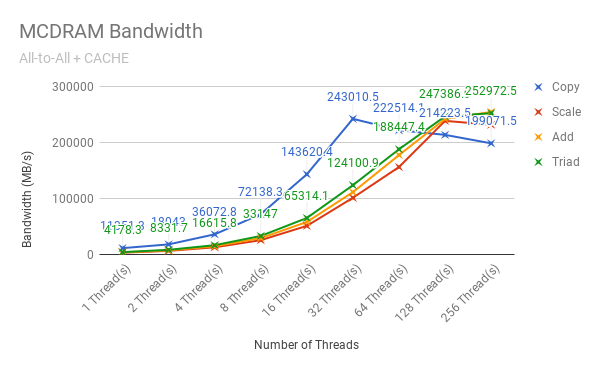
\includegraphics[width=\textwidth]{Results/mcdram_a2a_c_scaled.png}
    \caption{MCDRAM - Cache Mode - Scaled}
    \label{res:mcdram-a2a-c-scaled}
\end{figure}

\begin{figure}[!h]
    \centering
    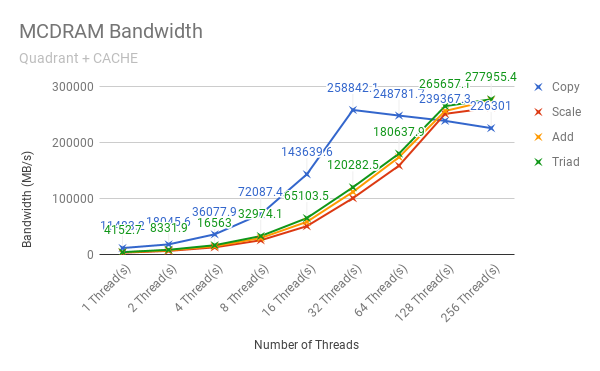
\includegraphics[width=\textwidth]{Results/mcdram_quad_c_scaled.png}
    \caption{MCDRAM - Cache Mode - Scaled}
    \label{res:mcdram-quad-c-scaled}
\end{figure}

\begin{figure}[!h]
    \centering
    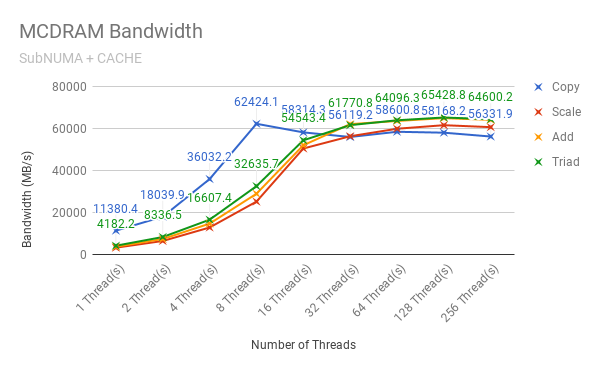
\includegraphics[width=\textwidth]{Results/mcdram_snc4_c_scaled.png}
    \caption{MCDRAM - Cache Mode - Scaled}
    \label{res:mcdram-snc4-c-scaled}
\end{figure}

\begin{figure}[!h]
    \centering
    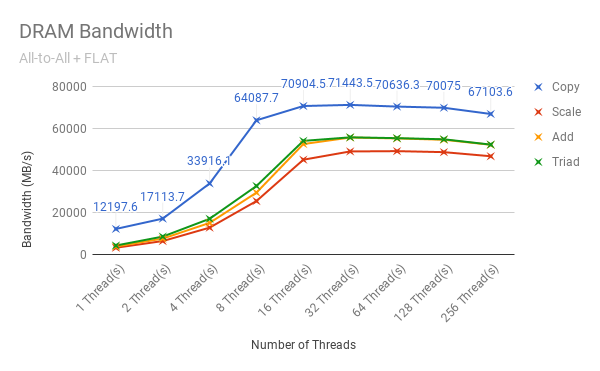
\includegraphics[width=\textwidth]{Results/dram_a2a_f_scaled.png}
    \caption{DRAM - Cache Mode - Scaled}
    \label{res:dram-a2a-f-scaled}
\end{figure}

\begin{figure}[!h]
    \centering
    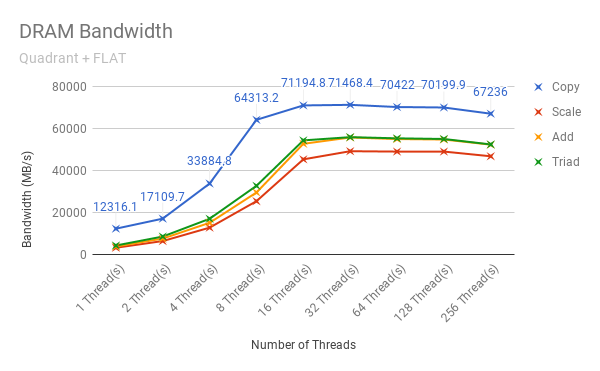
\includegraphics[width=\textwidth]{Results/dram_quad_f_scaled.png}
    \caption{DRAM - Cache Mode - Scaled}
    \label{res:dram-quad-f-scaled}
\end{figure}

\begin{figure}[!h]
    \centering
    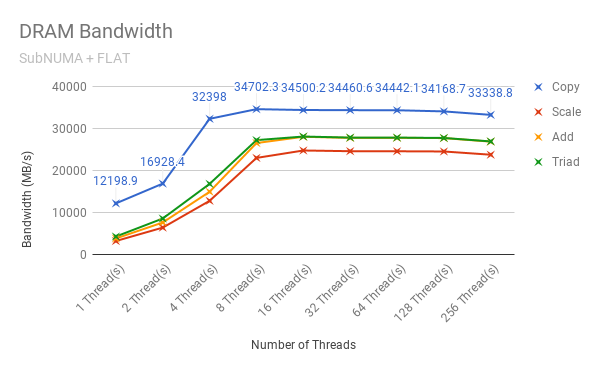
\includegraphics[width=\textwidth]{Results/dram_snc4_f_scaled.png}
    \caption{DRAM - Cache Mode - Scaled}
    \label{res:dram-snc4-f-scaled}
\end{figure}


\end{document}
